\begin{appendices}
    \chapter{MONKS' learning curves} % (fold)
    \label{cha:monks_learning_curves}
        Here we present the \textit{learning curves} for the three MONKS datasets. We have sampled these curves
        during the final tests on each dataset by plotting one of the 10 trails we used for building the
        statistics we presented in section \ref{sec:monks}, hence each plot presents a possible learning curve
        for the best hyperparameters' selection for each dataset. Alongside of the learning curves
        we also provide the \textit{accuracy plots} in order to show how the accuracy score progresses
        during the epochs, and the \textit{gradient's norm plots} in order to show the convergence
        rate. In the first subsections of both the SGD and the CG sections, we attach some plots in order to show
        the differences between the various models and to better compare their behaviour. Again, the plot are
        relative to one sampled execution between the 10 trails done.

        \section{Stochastic Gradient Descent} % (fold)
        \label{sec:stochastic_gradient_descent}
        % section stochastic_gradient_descent (end)

            \subsection{Comparisons} % (fold)
            \label{sub:comparisons}

            \begin{figure}[H]
                \centering
                \begin{subfigure}{0.40\textwidth}
                    \resizebox{\textwidth}{!}{
                        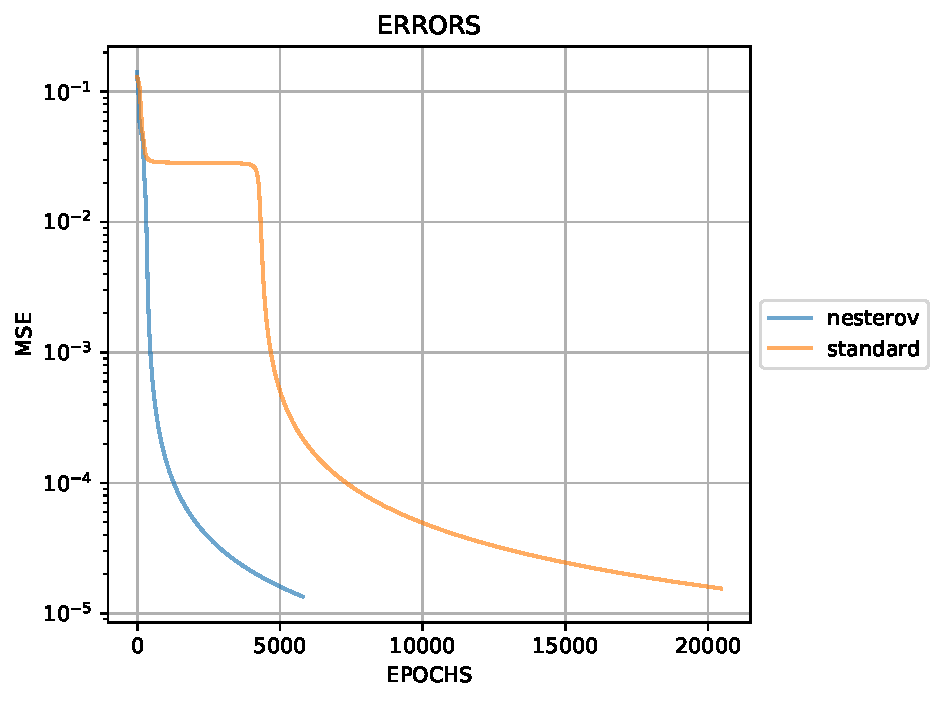
\includegraphics{img/1_mse_momentum.pdf}
                    }
                    \caption{}
                    \label{fig:monks_1_MSE_SGD}
                \end{subfigure}
                \begin{subfigure}{0.40\textwidth}
                    \resizebox{\textwidth}{!}{
                        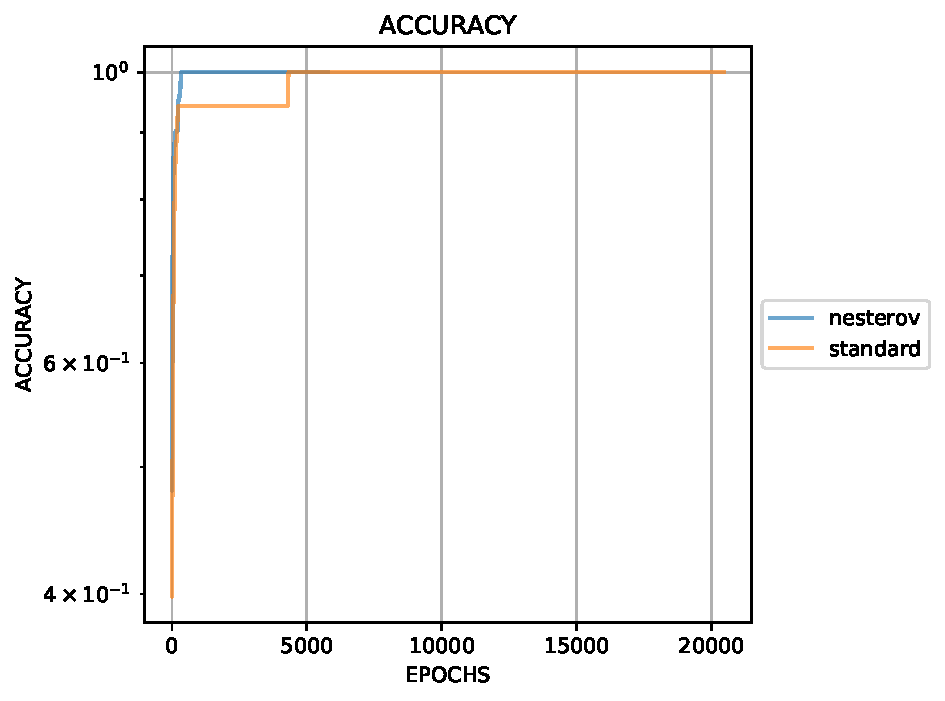
\includegraphics{img/1_accuracy_momentum.pdf}
                    }
                    \caption{}
                    \label{fig:monks_1_ACC_SGD}
                \end{subfigure}
                \caption{Example of a final learning, accuracy score curve on MONKS 1 with standard and nesterov momentum.}
                \label{fig:monks_1_SGD}
            \end{figure}

             \begin{figure}[H]
                \centering
                \begin{subfigure}{0.40\textwidth}
                    \resizebox{\textwidth}{!}{
                        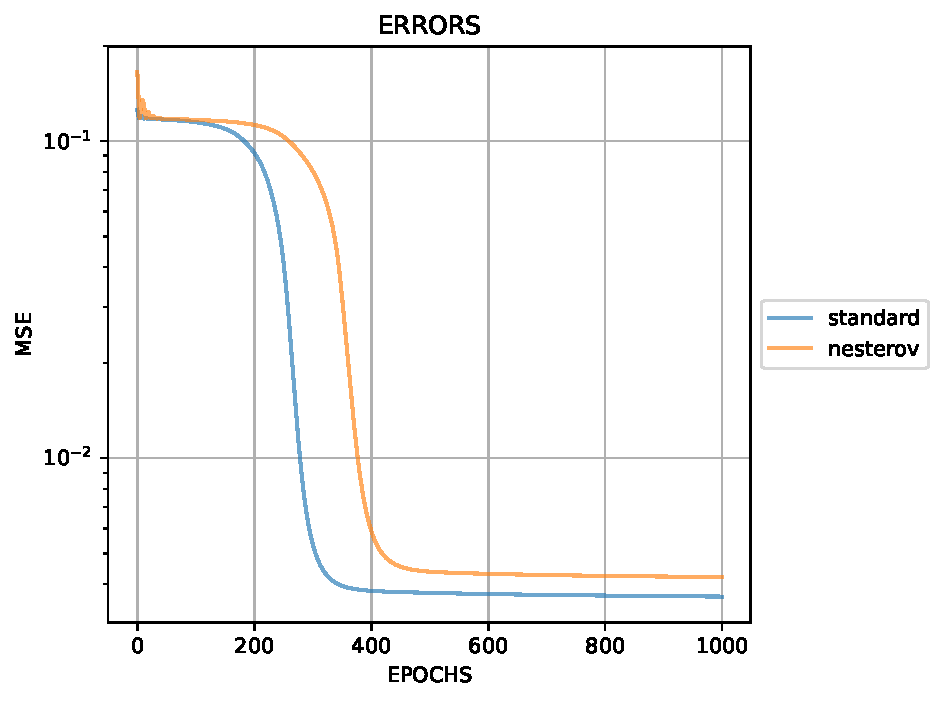
\includegraphics{img/2_mse_momentum.pdf}
                    }
                    \caption{}
                    \label{fig:monks_2_MSE_SGD}
                \end{subfigure}
                \begin{subfigure}{0.40\textwidth}
                    \resizebox{\textwidth}{!}{
                        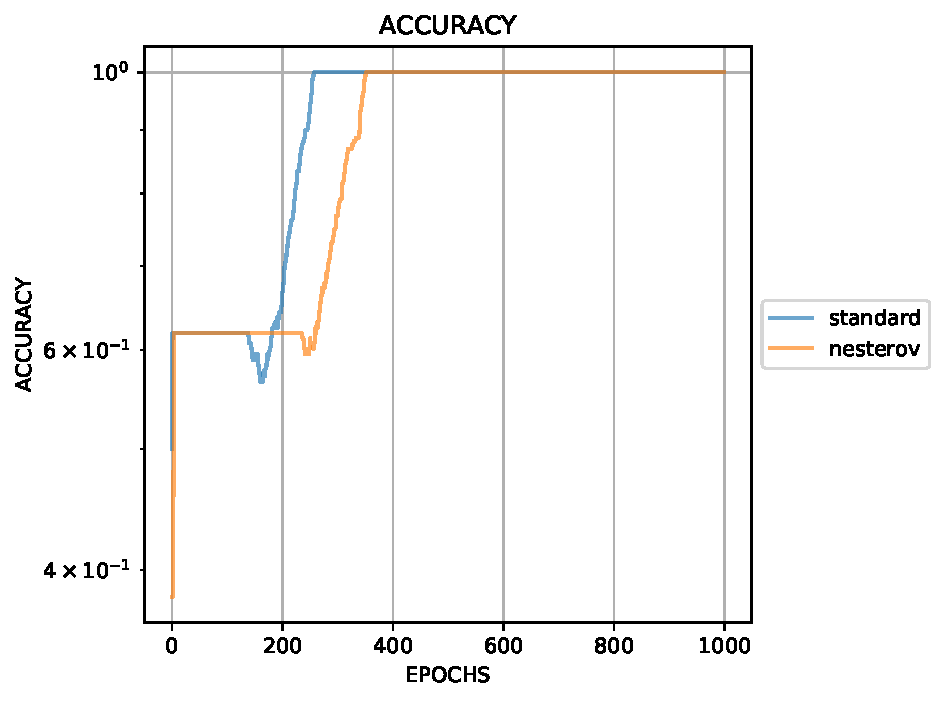
\includegraphics{img/2_accuracy_momentum.pdf}
                    }
                    \caption{}
                    \label{fig:monks_2_ACC_SGD}
                \end{subfigure}
                \caption{Example of a final learning, accuracy score curve on MONKS 2 with standard and nesterov momentum.}
                \label{fig:monks_2_SGD}
            \end{figure}

            \begin{figure}[H]
                \centering
                \begin{subfigure}{0.40\textwidth}
                    \resizebox{\textwidth}{!}{
                        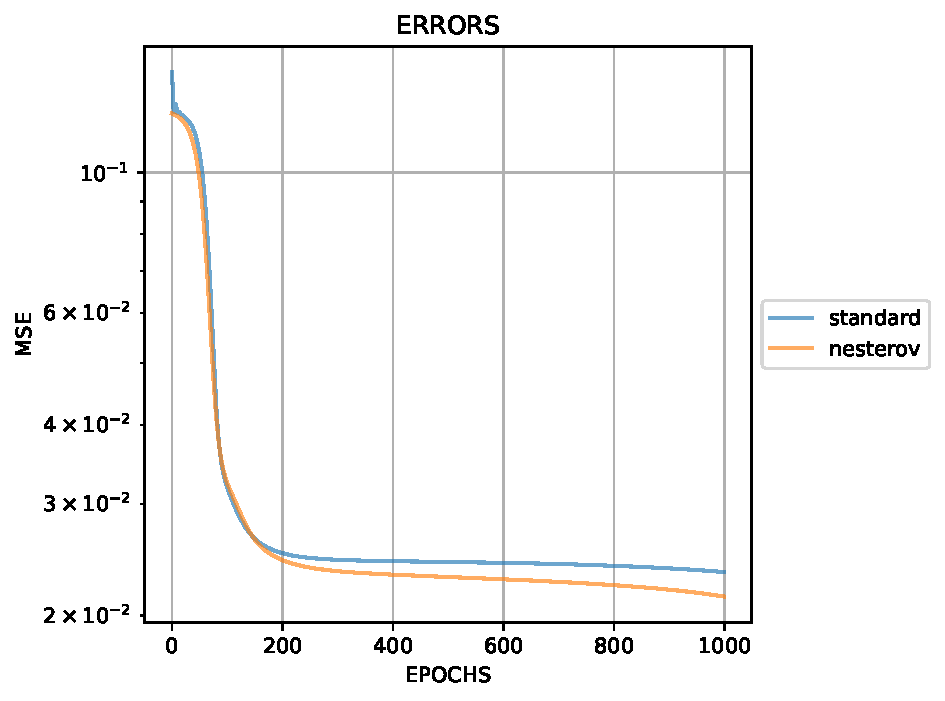
\includegraphics{img/3_mse_momentum.pdf}
                    }
                    \caption{}
                    \label{fig:monks_3_MSE_SGD}
                \end{subfigure}
                \begin{subfigure}{0.40\textwidth}
                    \resizebox{\textwidth}{!}{
                        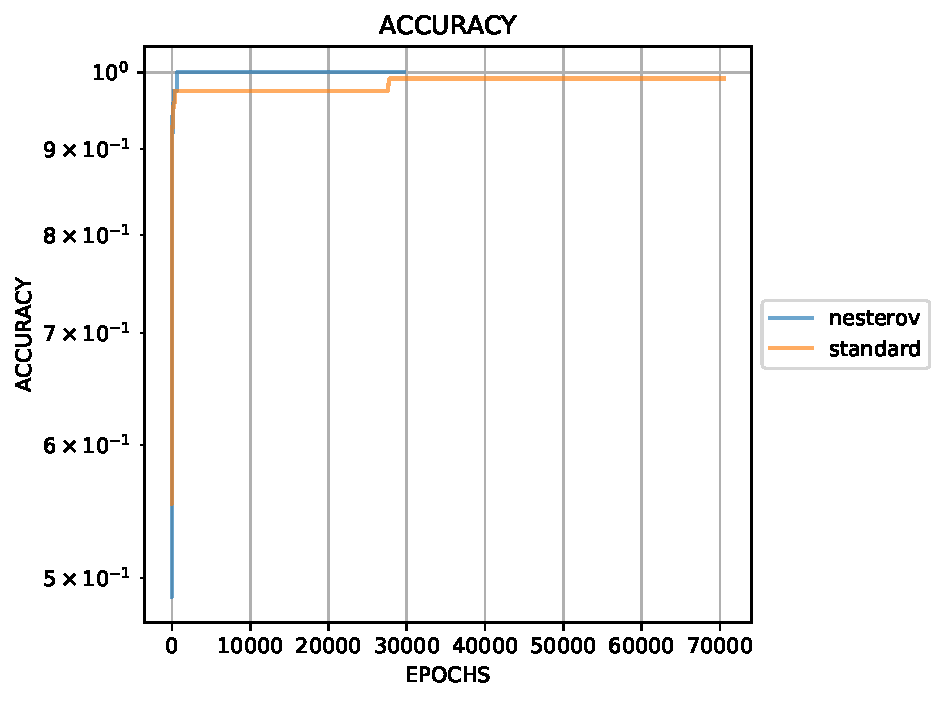
\includegraphics{img/3_accuracy_momentum.pdf}
                    }
                    \caption{}
                    \label{fig:monks_3_ACC_SGD}
                \end{subfigure}
                \caption{Example of a final learning, accuracy score curve on MONKS 3 with standard and nesterov momentum.}
                \label{fig:monks_3_SGD}
            \end{figure}

            \subsection{Standard momentum} % (fold)
            \label{sub:standard_momentum}

            \begin{figure}[H]
                \centering
                \begin{subfigure}{0.40\textwidth}
                    \resizebox{\textwidth}{!}{
                        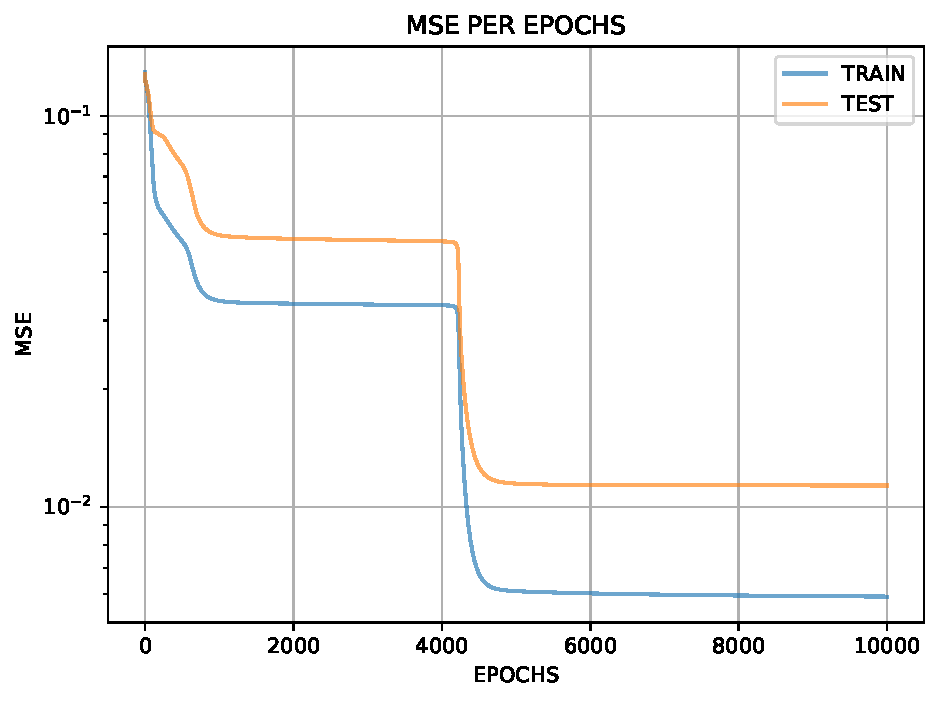
\includegraphics{img/SGD/sgd_mse_test_monks_1_standard.pdf}
                    }
                    \caption{}
                    \label{fig:monks_1_MSE_SGD}
                \end{subfigure}
                \begin{subfigure}{0.40\textwidth}
                    \resizebox{\textwidth}{!}{
                        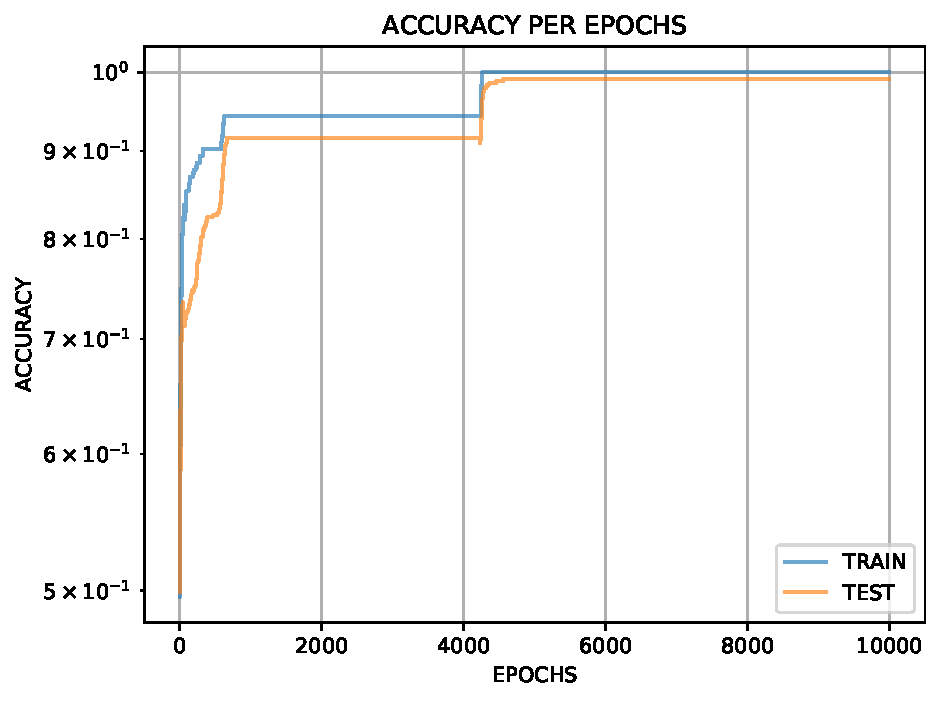
\includegraphics{img/SGD/sgd_accuracy_test_monks_1_standard.pdf}
                    }
                    \caption{}
                    \label{fig:monks_1_ACC_SGD}
                \end{subfigure}
                \begin{subfigure}{0.40\textwidth}
                    \resizebox{\textwidth}{!}{
                        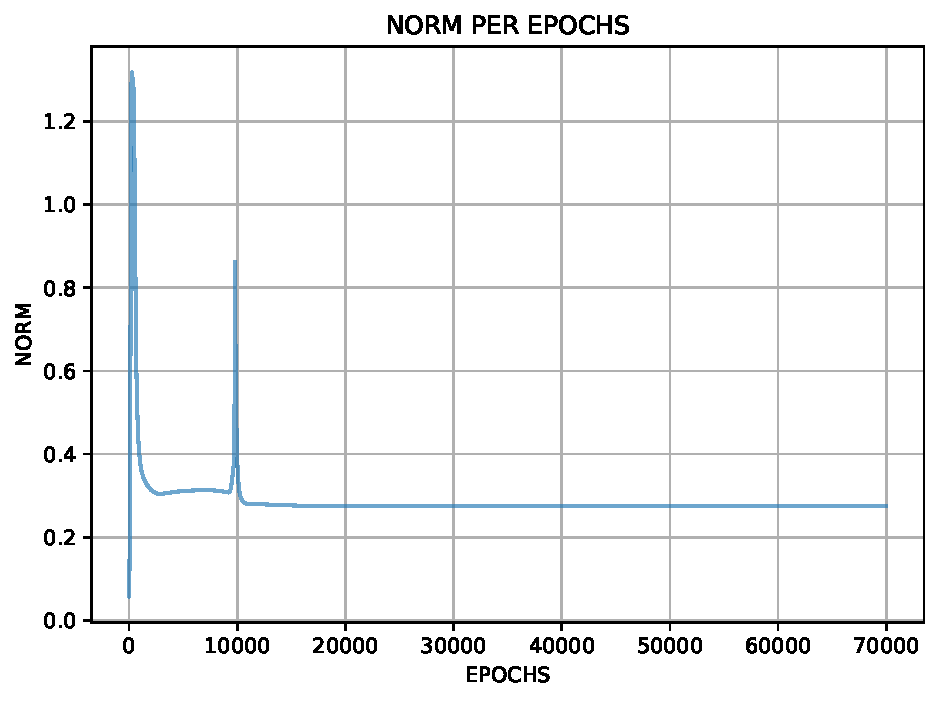
\includegraphics{img/SGD/sgd_norm_test_monks_1_standard.pdf}
                    }
                    \caption{}
                    \label{fig:monks_1_NORM_SGD}
                \end{subfigure}
                \caption{Example of a final learning, accuracy score curve and
                convergence rate curve on MONKS 1 with standard momentum.}
                \label{fig:monks_1_SGD}
            \end{figure}

            \begin{figure}[H]
                \centering
                \begin{subfigure}{0.40\textwidth}
                    \resizebox{\textwidth}{!}{
                        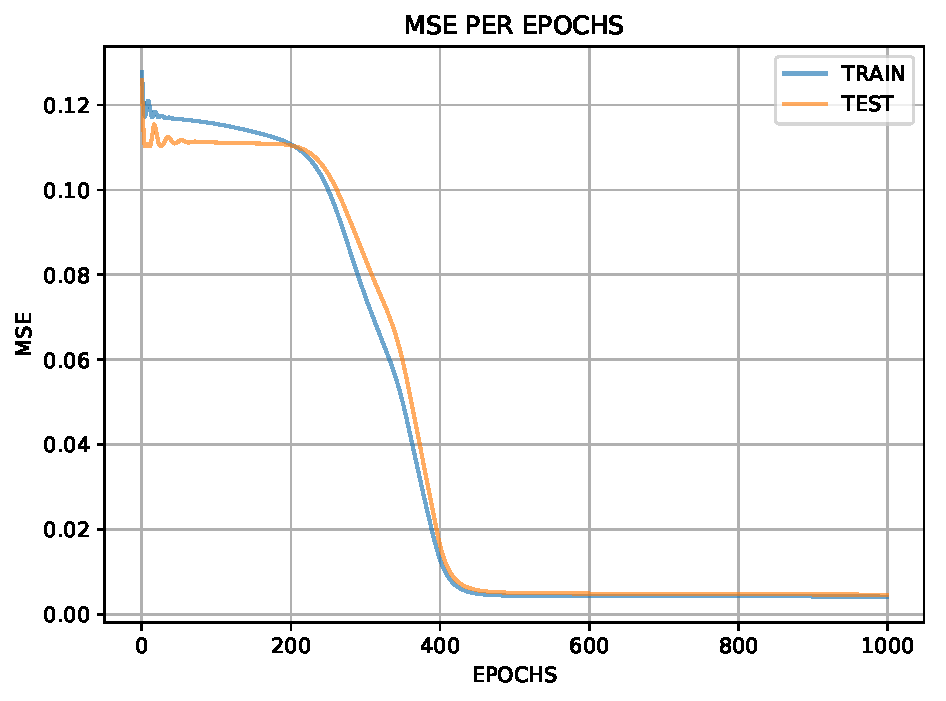
\includegraphics{img/SGD/sgd_mse_test_monks_2_standard.pdf}
                    }
                    \caption{}
                    \label{fig:monks_2_MSE_SGD}
                \end{subfigure}
                \begin{subfigure}{0.40\textwidth}
                    \resizebox{\textwidth}{!}{
                        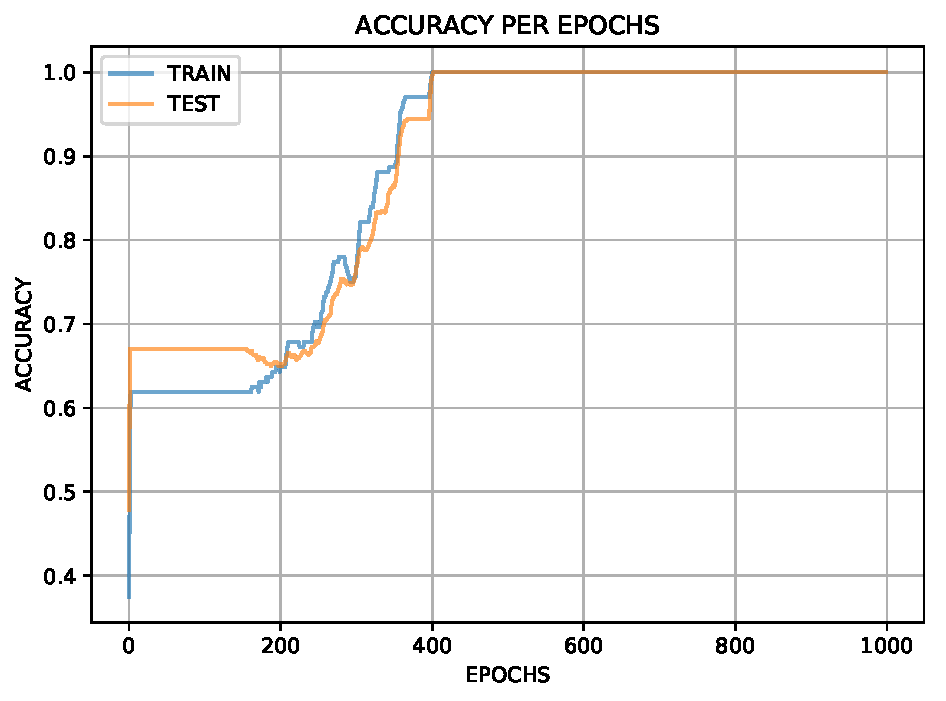
\includegraphics{img/SGD/sgd_accuracy_test_monks_2_standard.pdf}
                    }
                    \caption{}
                    \label{fig:monks_2_ACC_SGD}
                \end{subfigure}
                \begin{subfigure}{0.40\textwidth}
                    \resizebox{\textwidth}{!}{
                        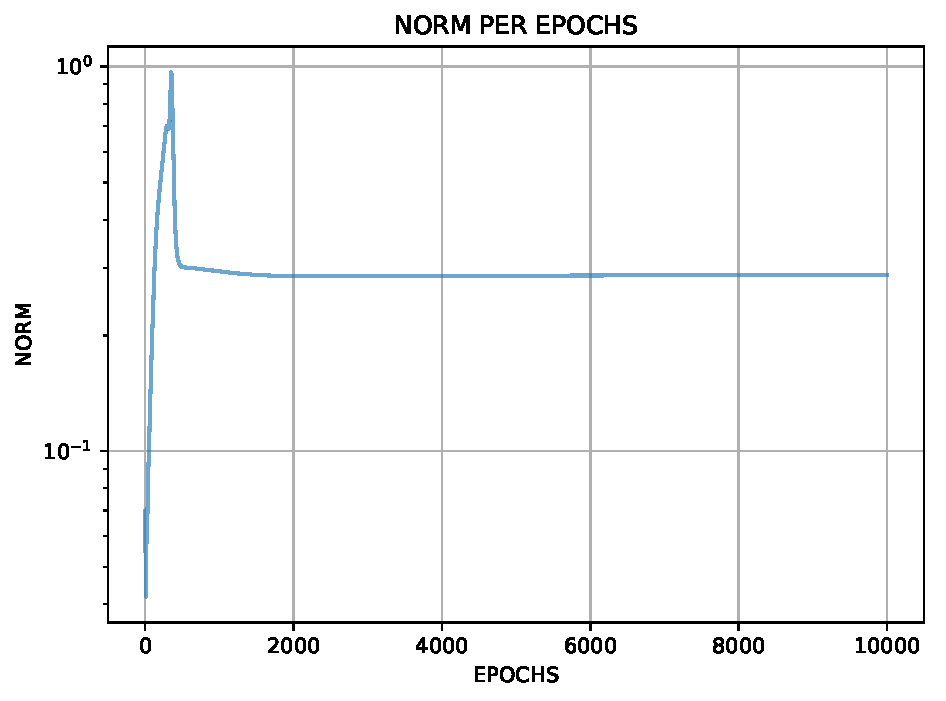
\includegraphics{img/SGD/sgd_norm_test_monks_2_standard.pdf}
                    }
                    \caption{}
                    \label{fig:monks_2_NORM_SGD}
                \end{subfigure}
                \caption{Example of a final learning, accuracy score curve and
                convergence rate curve on MONKS 2 with standard momentum.}
                \label{fig:monks_2_SGD}
            \end{figure}

            \begin{figure}[H]
                \centering
                \begin{subfigure}{0.40\textwidth}
                    \resizebox{\textwidth}{!}{
                        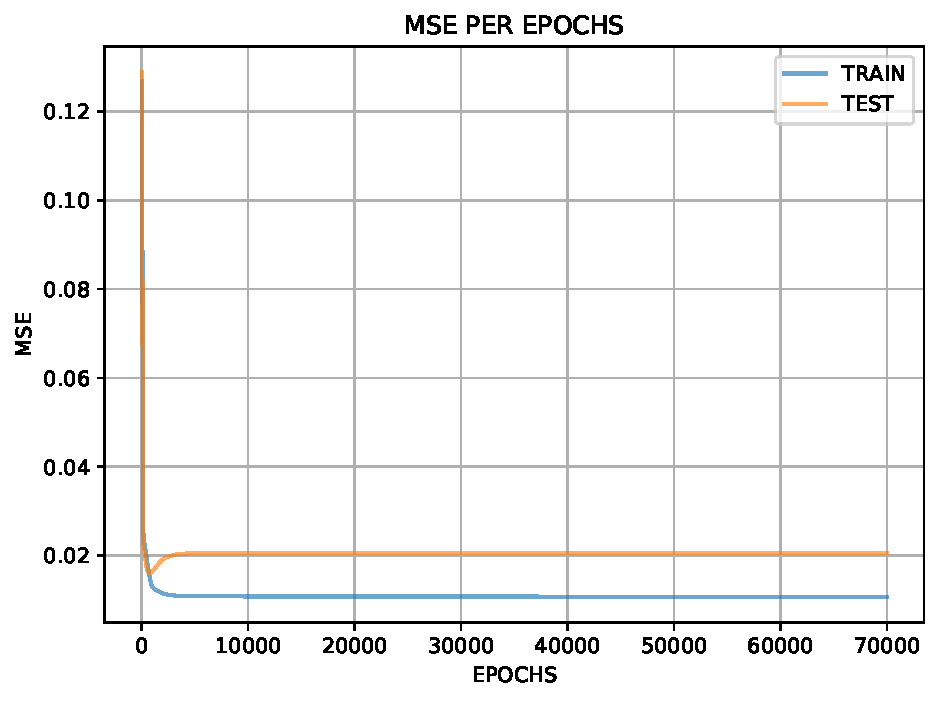
\includegraphics{img/SGD/sgd_mse_test_monks_3_standard.pdf}
                    }
                    \caption{}
                    \label{fig:monks_3_MSE_SGD}
                \end{subfigure}
                \begin{subfigure}{0.40\textwidth}
                    \resizebox{\textwidth}{!}{
                        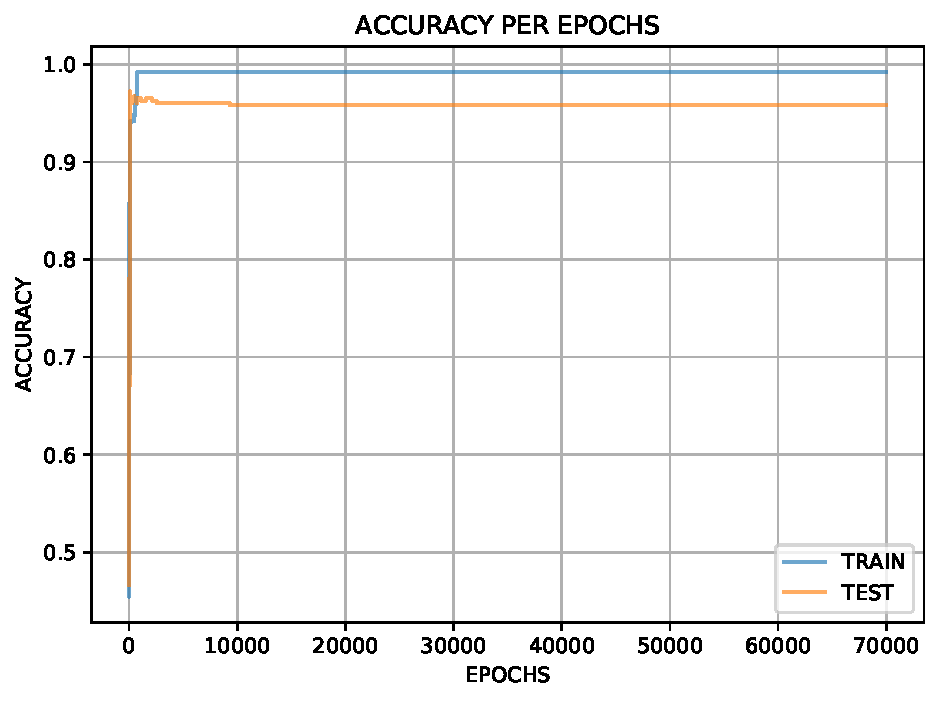
\includegraphics{img/SGD/sgd_accuracy_test_monks_3_standard.pdf}
                    }
                    \caption{}
                    \label{fig:monks_3_ACC_SGD}
                \end{subfigure}
                \begin{subfigure}{0.40\textwidth}
                    \resizebox{\textwidth}{!}{
                        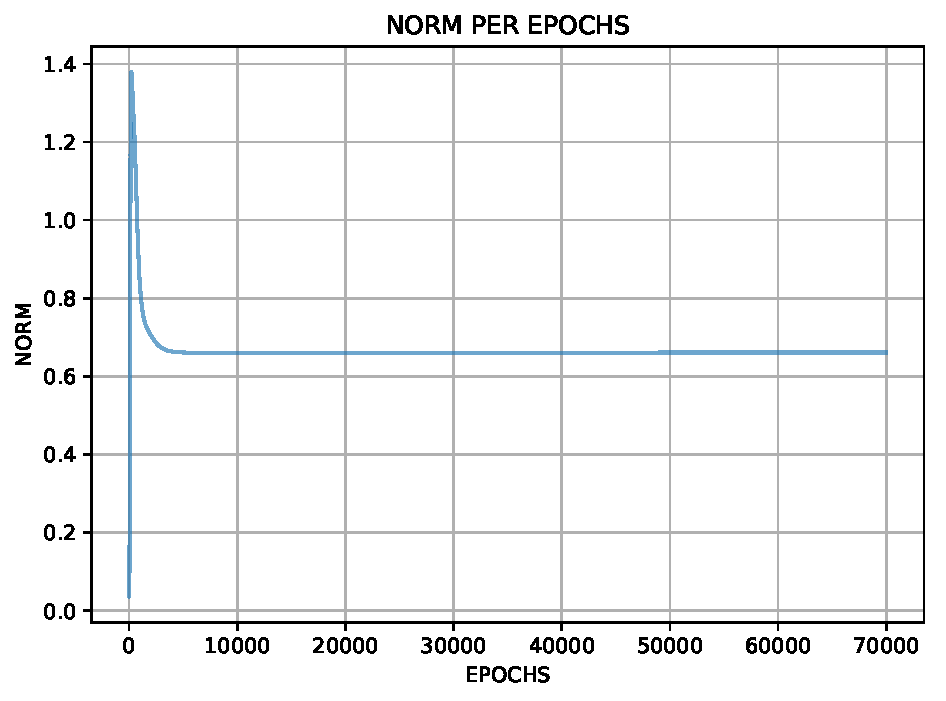
\includegraphics{img/SGD/sgd_norm_test_monks_3_standard.pdf}
                    }
                    \caption{}
                    \label{fig:monks_3_NORM_SGD}
                \end{subfigure}
                \caption{Example of a final learning, accuracy score curve and
                convergence rate curve on MONKS 3 with standard momentum.}
                \label{fig:monks_3_SGD}
            \end{figure}

            % subsection standard_momentum (end)

            \subsection{Nesterov's momentum} % (fold)
            \label{sub:nesterov_s_momentum}

            \begin{figure}[H]
                \centering
                \begin{subfigure}{0.40\textwidth}
                    \resizebox{\textwidth}{!}{
                        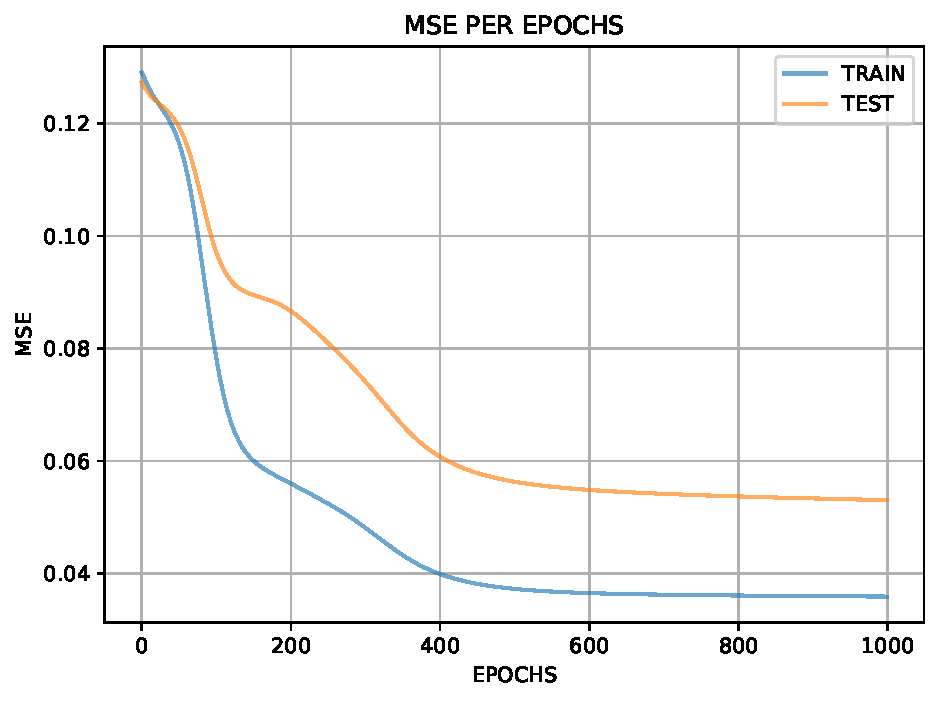
\includegraphics{img/SGD/sgd_mse_test_monks_1_nesterov.pdf}
                    }
                    \caption{}
                    \label{fig:monks_1_MSE_SGD}
                \end{subfigure}
                \begin{subfigure}{0.40\textwidth}
                    \resizebox{\textwidth}{!}{
                        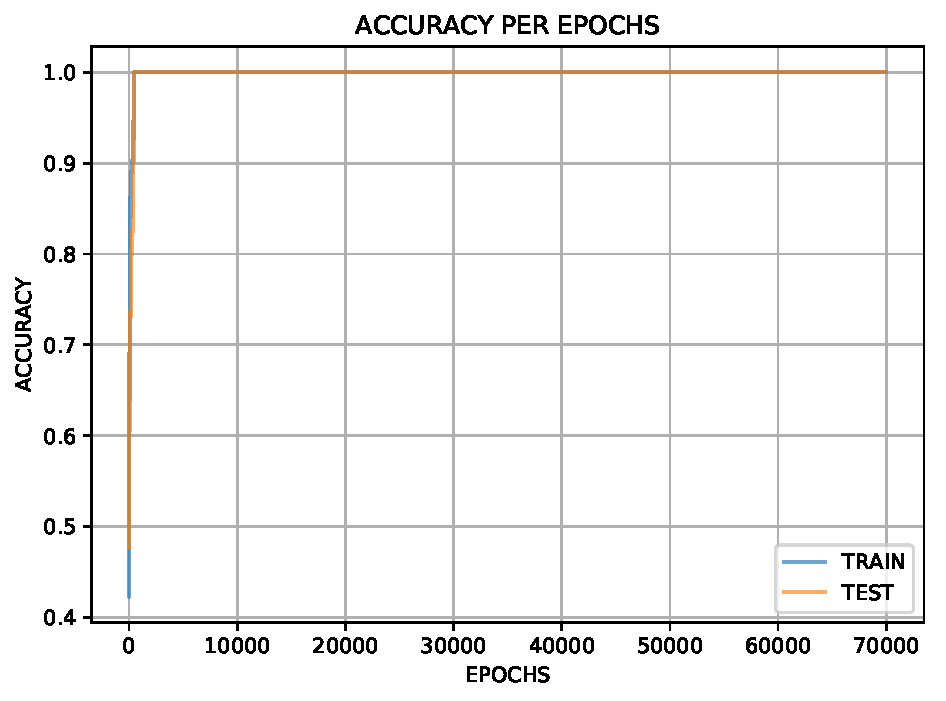
\includegraphics{img/SGD/sgd_accuracy_test_monks_1_nesterov.pdf}
                    }
                    \caption{}
                    \label{fig:monks_1_ACC_SGD}
                \end{subfigure}
                \begin{subfigure}{0.40\textwidth}
                    \resizebox{\textwidth}{!}{
                        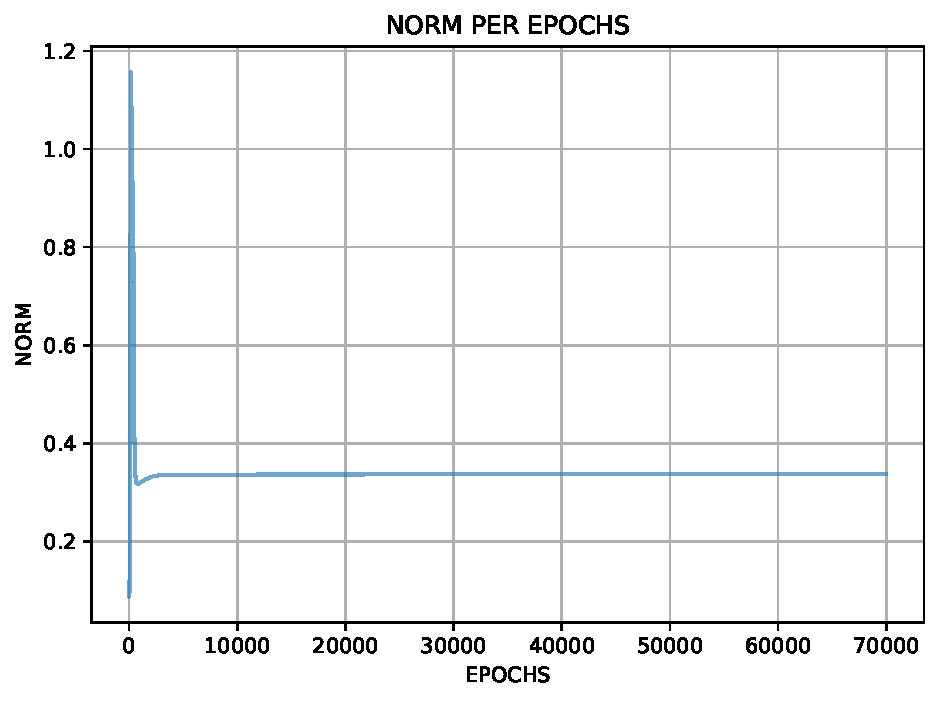
\includegraphics{img/SGD/sgd_norm_test_monks_1_nesterov.pdf}
                    }
                    \caption{}
                    \label{fig:monks_1_NORM_SGD}
                \end{subfigure}
                \caption{Example of a final learning, accuracy score curve and
                convergence rate curve on MONKS 1 with Nesterov's momentum.}
                \label{fig:monks_1_SGD}
            \end{figure}

            \begin{figure}[H]
                \centering
                \begin{subfigure}{0.40\textwidth}
                    \resizebox{\textwidth}{!}{
                        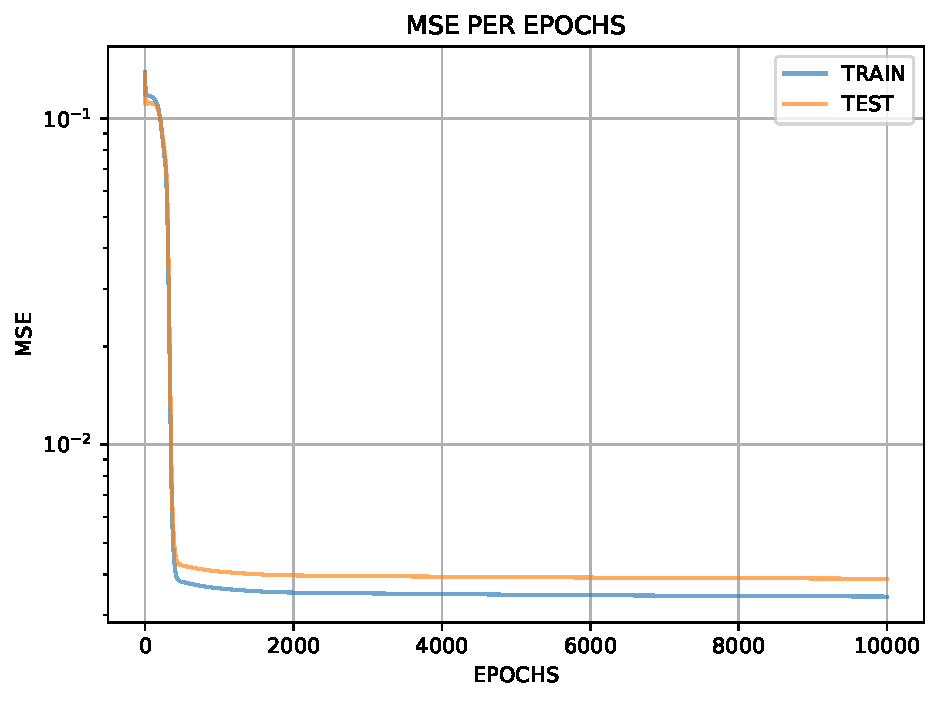
\includegraphics{img/SGD/sgd_mse_test_monks_2_nesterov.pdf}
                    }
                    \caption{}
                    \label{fig:monks_2_MSE_SGD}
                \end{subfigure}
                \begin{subfigure}{0.40\textwidth}
                    \resizebox{\textwidth}{!}{
                        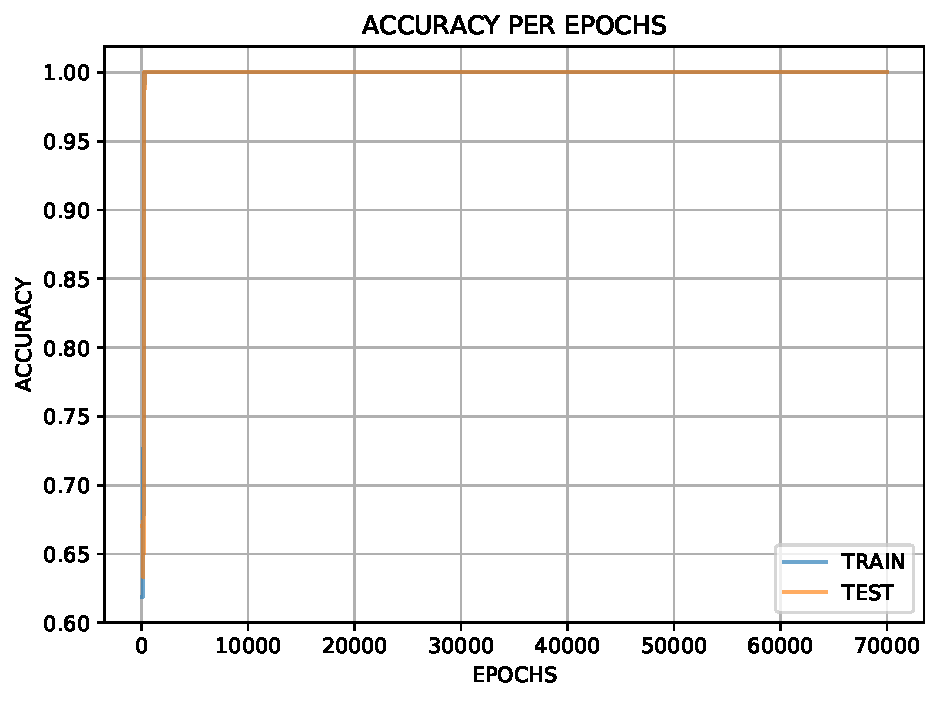
\includegraphics{img/SGD/sgd_accuracy_test_monks_2_nesterov.pdf}
                    }
                    \caption{}
                    \label{fig:monks_2_ACC_SGD}
                \end{subfigure}
                \begin{subfigure}{0.40\textwidth}
                    \resizebox{\textwidth}{!}{
                        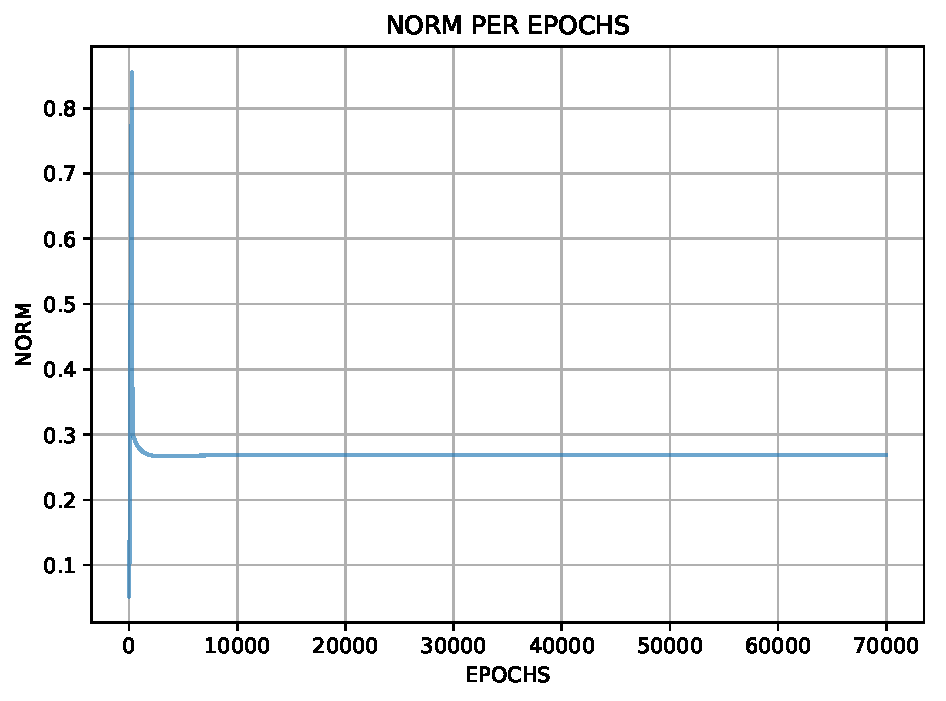
\includegraphics{img/SGD/sgd_norm_test_monks_2_nesterov.pdf}
                    }
                    \caption{}
                    \label{fig:monks_2_NORM_SGD}
                \end{subfigure}
                \caption{Example of a final learning, accuracy score curve and
                convergence rate curve on MONKS 2 with Nesterov's momentum.}
                \label{fig:monks_1_SGD}
            \end{figure}

            \begin{figure}[H]
                \centering
                \begin{subfigure}{0.40\textwidth}
                    \resizebox{\textwidth}{!}{
                        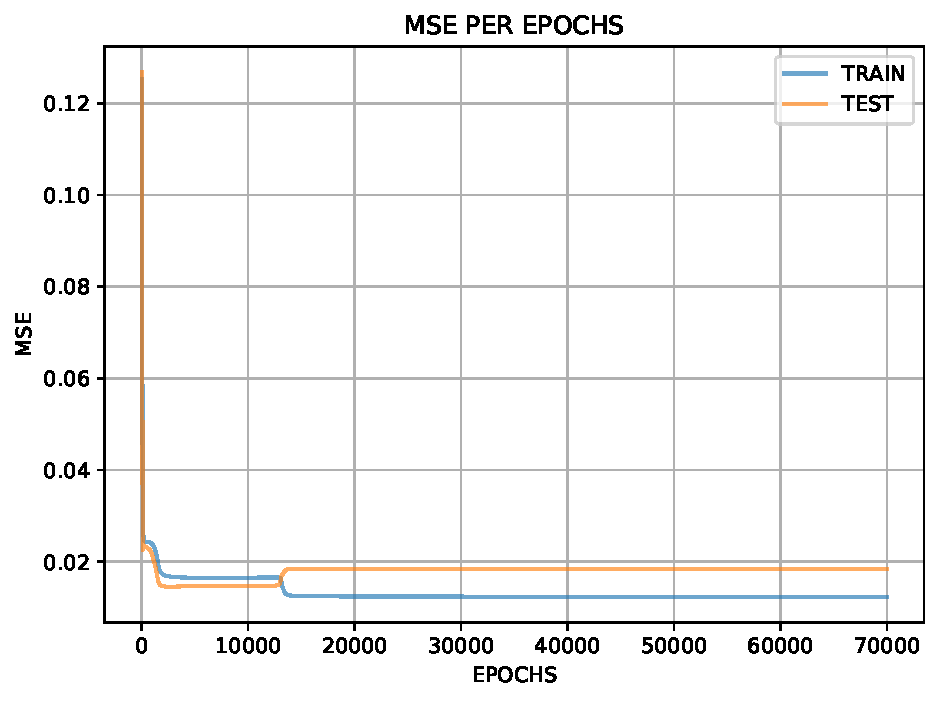
\includegraphics{img/SGD/sgd_mse_test_monks_3_nesterov.pdf}
                    }
                    \caption{}
                    \label{fig:monks_3_MSE_SGD}
                \end{subfigure}
                \begin{subfigure}{0.40\textwidth}
                    \resizebox{\textwidth}{!}{
                        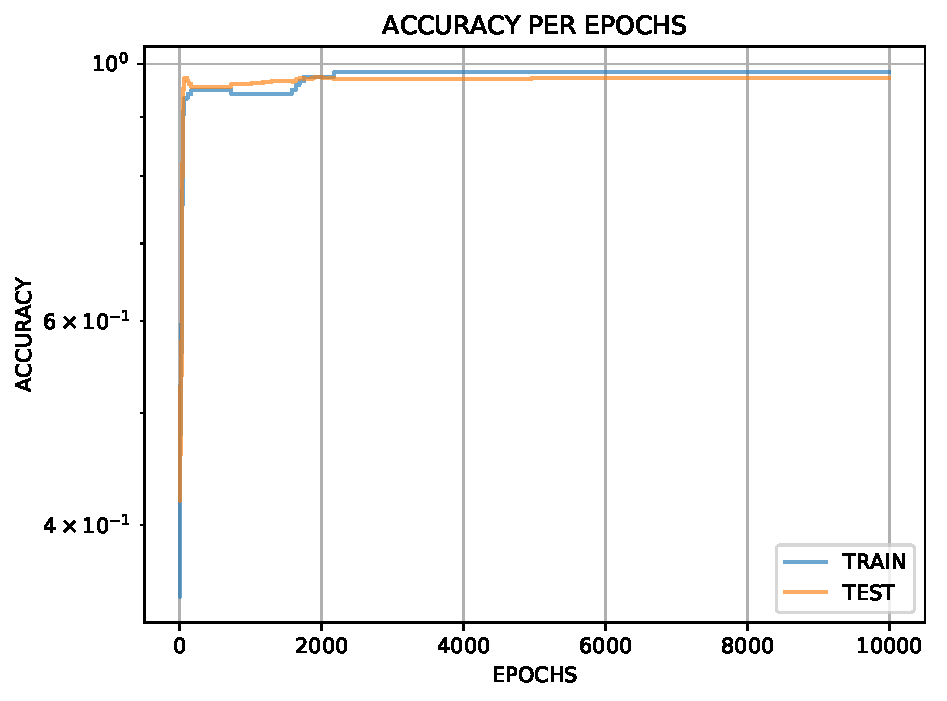
\includegraphics{img/SGD/sgd_accuracy_test_monks_3_nesterov.pdf}
                    }
                    \caption{}
                    \label{fig:monks_3_ACC_SGD}
                \end{subfigure}
                \begin{subfigure}{0.40\textwidth}
                    \resizebox{\textwidth}{!}{
                        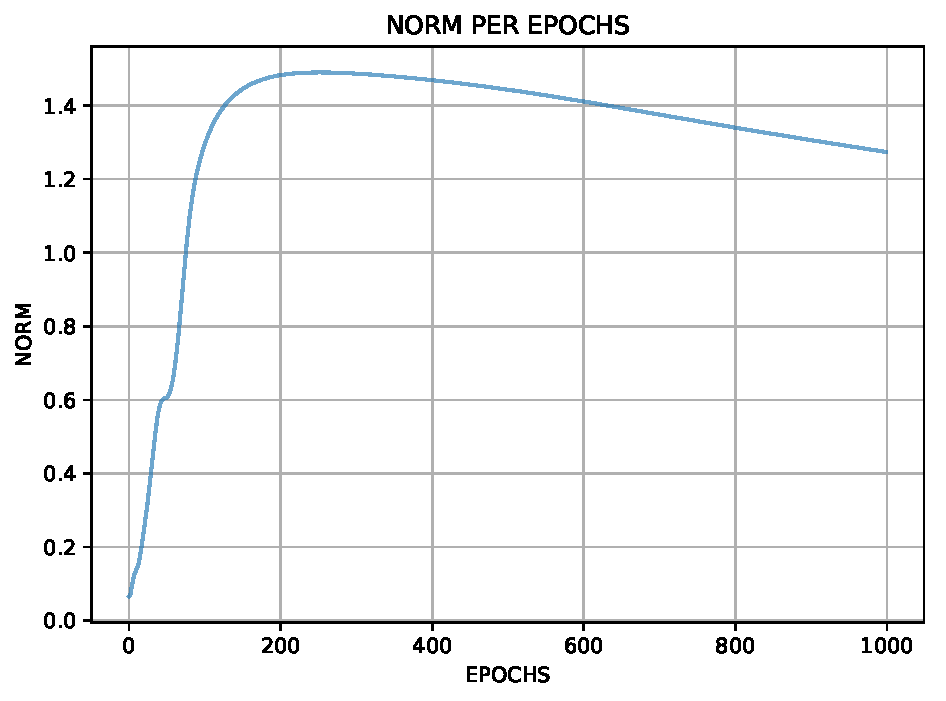
\includegraphics{img/SGD/sgd_norm_test_monks_3_nesterov.pdf}
                    }
                    \caption{}
                    \label{fig:monks_3_NORM_SGD}
                \end{subfigure}
                \caption{Example of a final learning, accuracy score curve and
                convergence rate curve on MONKS 3 with Nesterov's momentum.}
                \label{fig:monks_1_SGD}
            \end{figure}

            % subsection nesterov_s_momentum (end)

         \section{Conjugate Gradient Methods} % (fold)
         \label{sec:conjugate_gradient_methods}
            \subsection{Comparisons} % (fold)
            \label{sub:comparisons}

            \begin{figure}[H]
                \centering
                \begin{subfigure}{0.4\textwidth}
                    \resizebox{\textwidth}{!}{
                        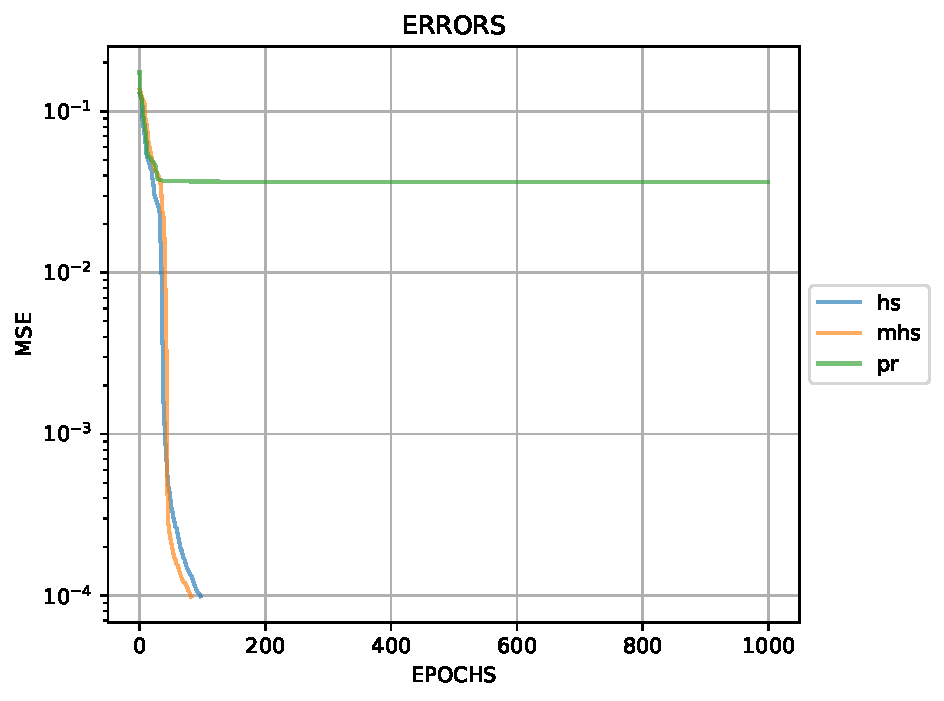
\includegraphics{img/1_mse_beta.pdf}
                    }
                    \caption{}
                    \label{fig:monks_1_MSE_CGD}
                \end{subfigure}
                \begin{subfigure}{0.4\textwidth}
                    \resizebox{\textwidth}{!}{
                        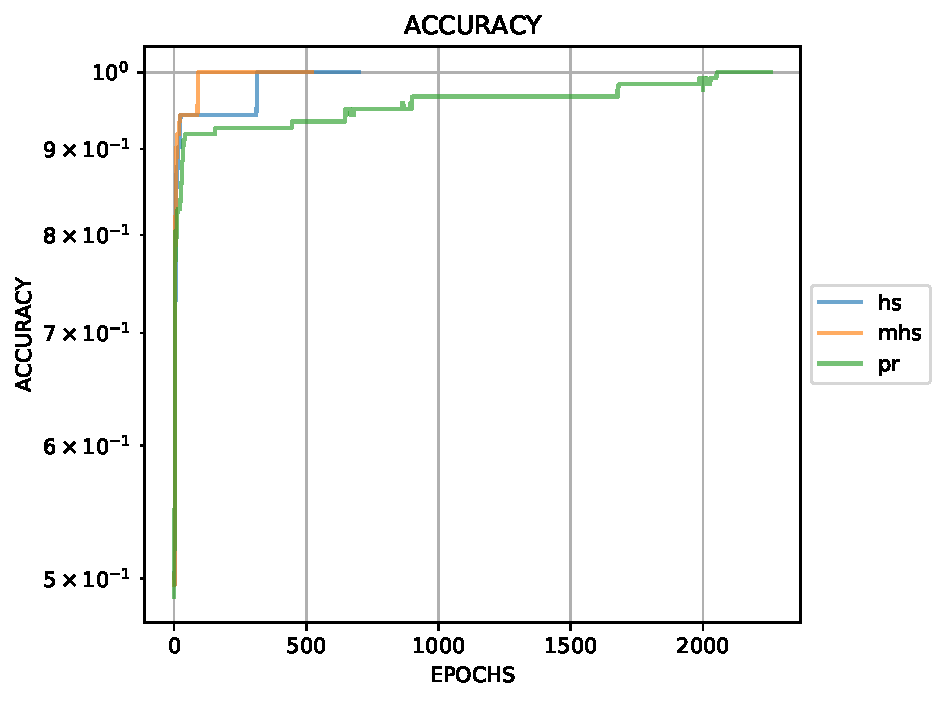
\includegraphics{img/1_accuracy_beta.pdf}
                    }
                    \caption{}
                    \label{fig:monks_1_ACC_CGD}
                \end{subfigure}
                \caption{Example of a final learning, accuracy score curve on MONKS 1 with different beta methods.}
                \label{fig:monks_1_CGD}
            \end{figure}

             \begin{figure}[H]
                \centering
                \begin{subfigure}{0.40\textwidth}
                    \resizebox{\textwidth}{!}{
                        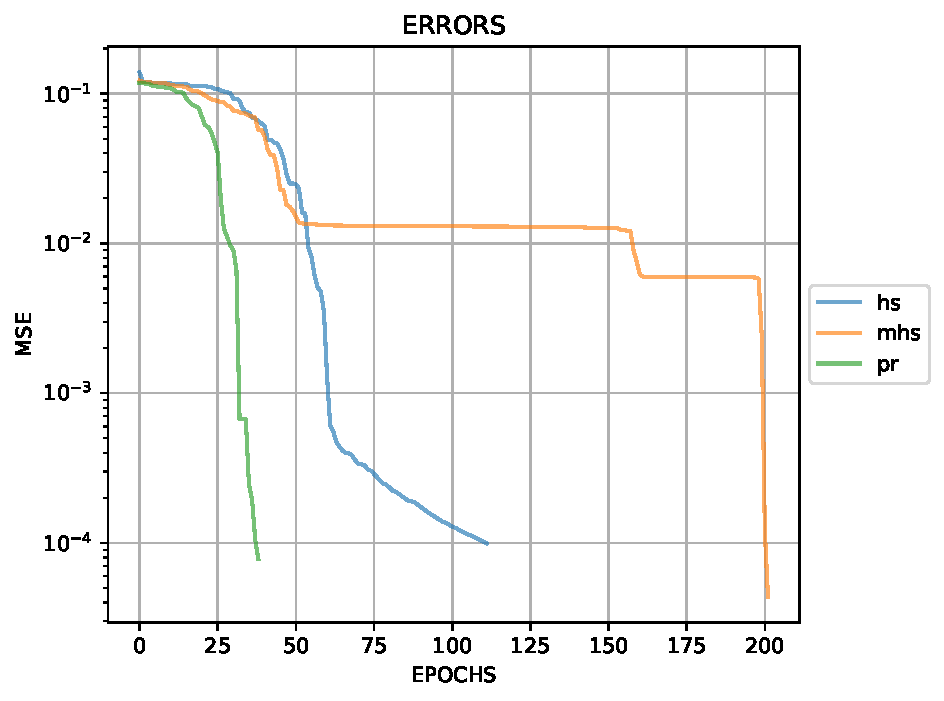
\includegraphics{img/2_mse_beta.pdf}
                    }
                    \caption{}
                    \label{fig:monks_2_MSE_CGD}
                \end{subfigure}
                \begin{subfigure}{0.40\textwidth}
                    \resizebox{\textwidth}{!}{
                        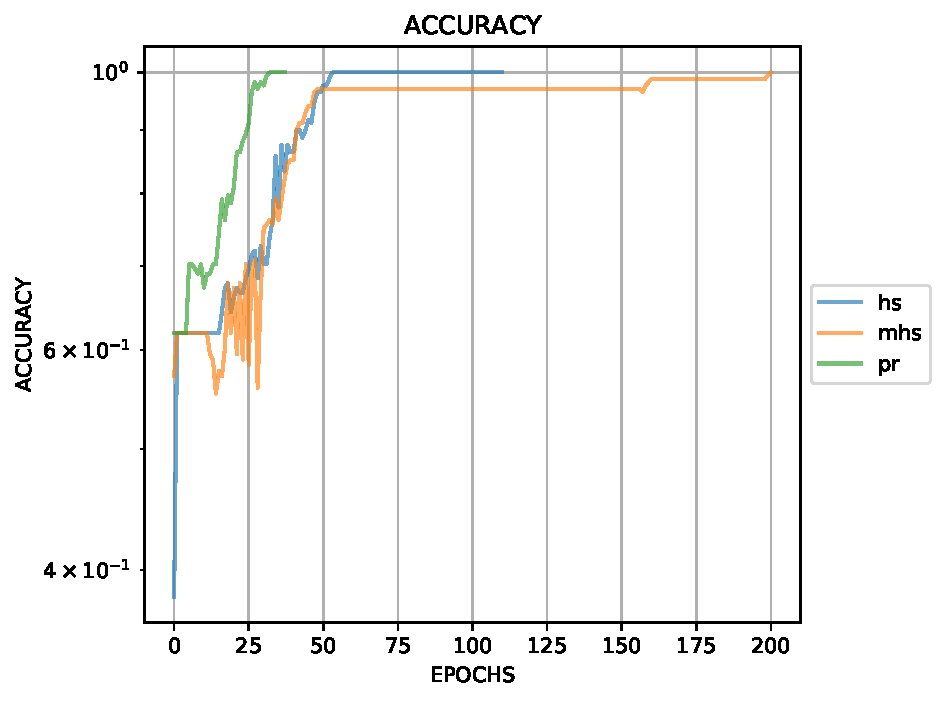
\includegraphics{img/2_accuracy_beta.pdf}
                    }
                    \caption{}
                    \label{fig:monks_2_ACC_CGD}
                \end{subfigure}
                \caption{Example of a final learning, accuracy score curve on MONKS 2 with different beta methods.}
                \label{fig:monks_2_CGD}
            \end{figure}

            \begin{figure}[H]
                \centering
                \begin{subfigure}{0.40\textwidth}
                    \resizebox{\textwidth}{!}{
                        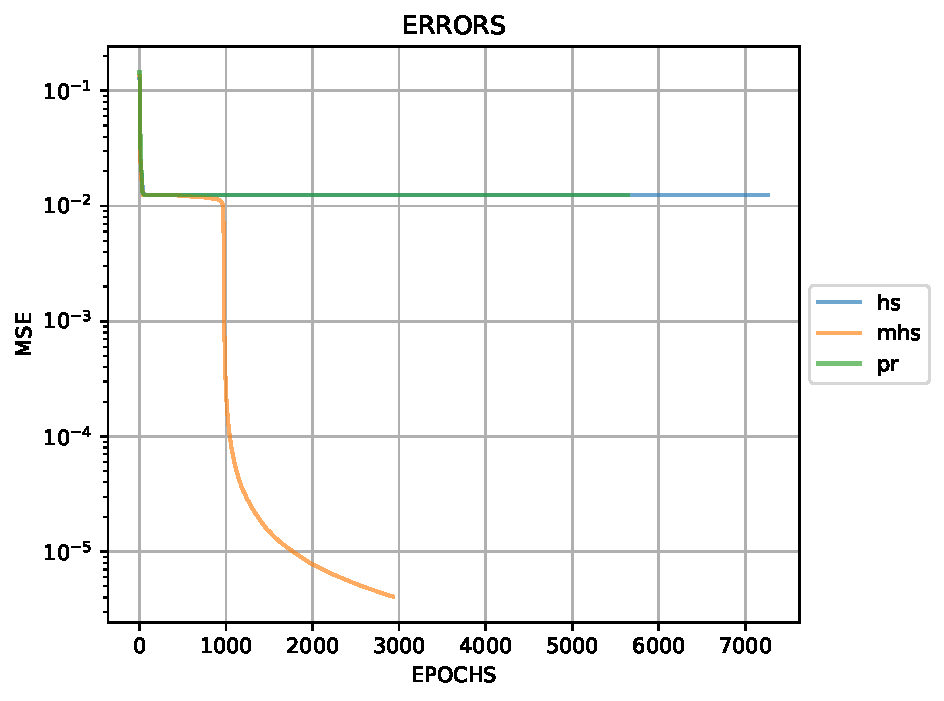
\includegraphics{img/3_mse_beta.pdf}
                    }
                    \caption{}
                    \label{fig:monks_3_MSE_CGD}
                \end{subfigure}
                \begin{subfigure}{0.40\textwidth}
                    \resizebox{\textwidth}{!}{
                        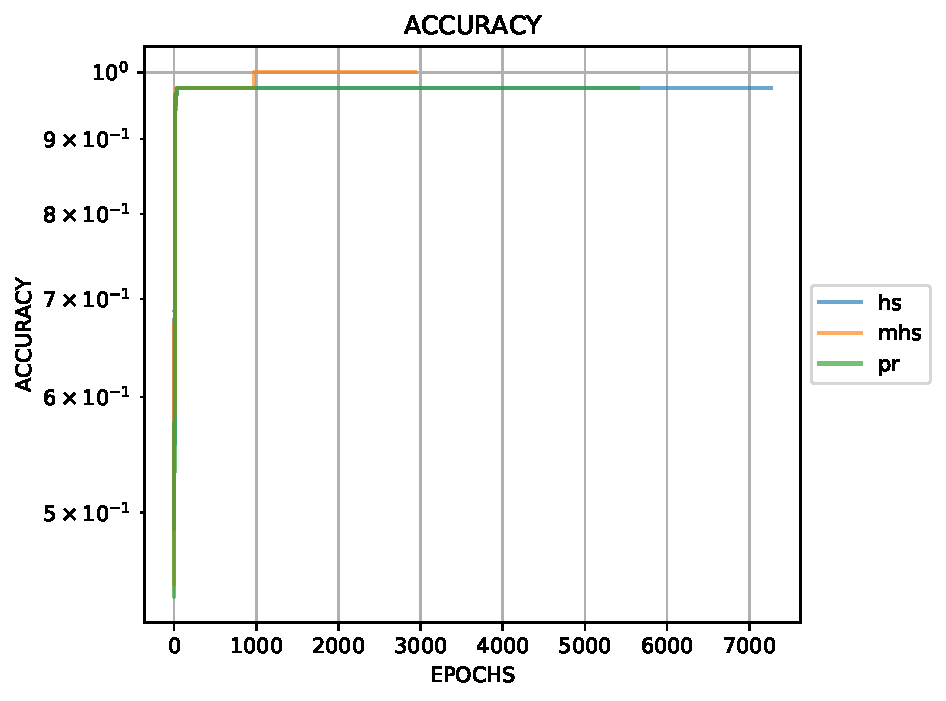
\includegraphics{img/3_accuracy_beta.pdf}
                    }
                    \caption{}
                    \label{fig:monks_3_ACC_CGD}
                \end{subfigure}
                \caption{Example of a final learning, accuracy score curve on MONKS 3 with different beta methods.}
                \label{fig:monks_3_CGD}
            \end{figure}

            \subsection{$MHS^+$} % (fold)
            \label{sub:mhs}

                \begin{figure}[H]
                \centering
                \begin{subfigure}{0.40\textwidth}
                    \resizebox{\textwidth}{!}{
                        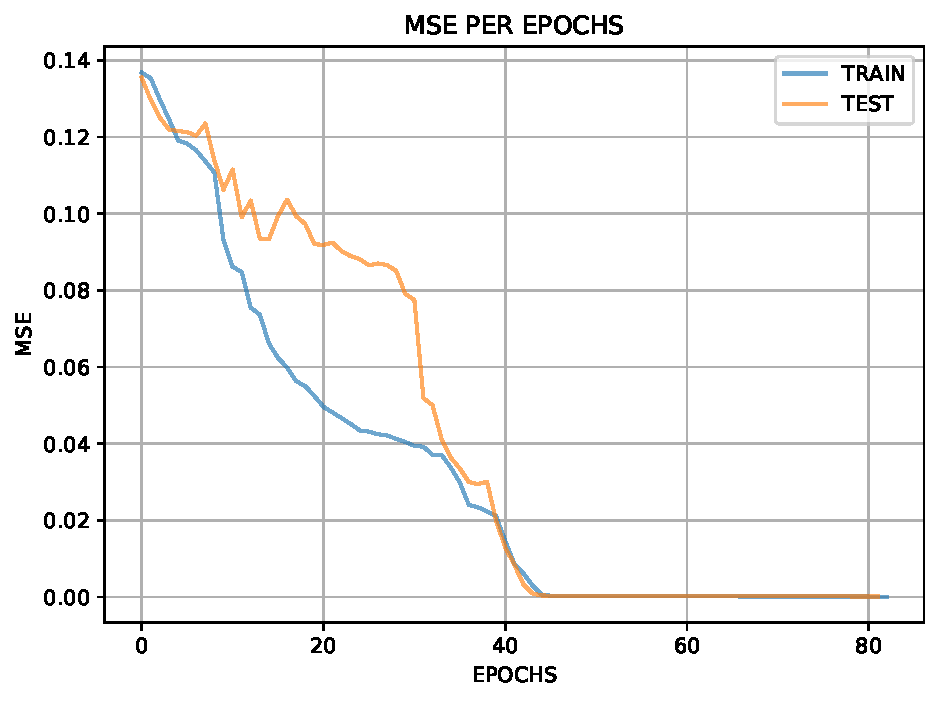
\includegraphics{img/CGD/MHS/cgd_mse_test_mhs_monks_1.pdf}
                    }
                    \caption{}
                    \label{fig:monks_1_MSE_CGD}
                \end{subfigure}
                \begin{subfigure}{0.40\textwidth}
                    \resizebox{\textwidth}{!}{
                        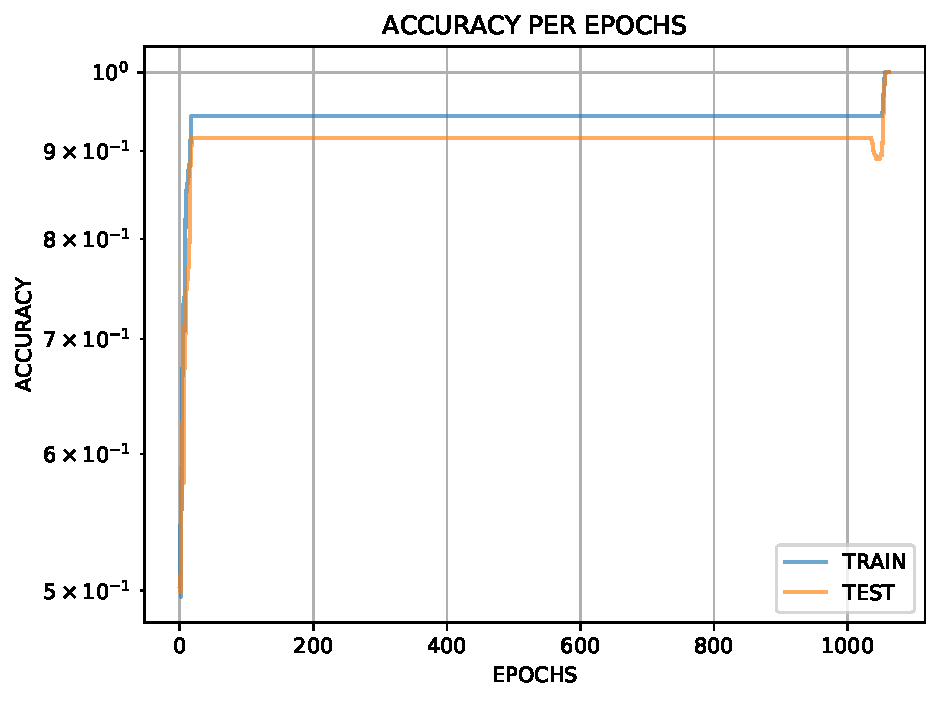
\includegraphics{img/CGD/MHS/cgd_accuracy_test_mhs_monks_1.pdf}
                    }
                    \caption{}
                    \label{fig:monks_1_ACC_CGD}
                \end{subfigure}
                \begin{subfigure}{0.40\textwidth}
                    \resizebox{\textwidth}{!}{
                        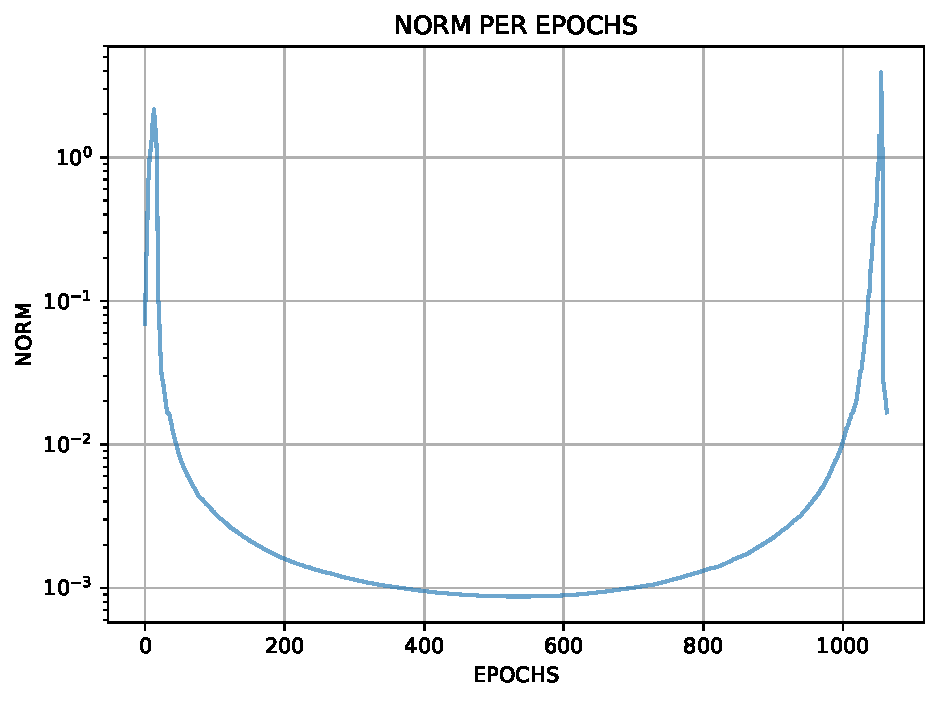
\includegraphics{img/CGD/MHS/cgd_norm_test_mhs_monks_1.pdf}
                    }
                    \caption{}
                    \label{fig:monks_1_NORM_CGD}
                \end{subfigure}
                \caption{Example of a final learning, accuracy score curve and
                convergence rate curve on MONKS 1 with $MHS^+$ method.}
                \label{fig:monks_1_CGD}
            \end{figure}

            \begin{figure}[H]
                \centering
                \begin{subfigure}{0.40\textwidth}
                    \resizebox{\textwidth}{!}{
                        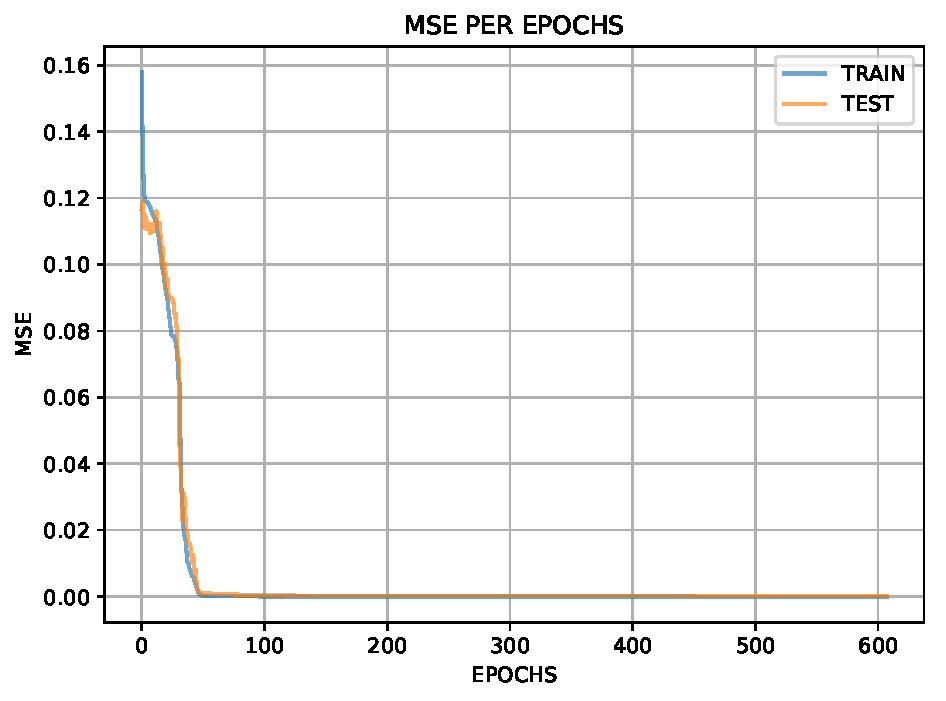
\includegraphics{img/CGD/MHS/cgd_mse_test_mhs_monks_2.pdf}
                    }
                    \caption{}
                    \label{fig:monks_2_MSE_CGD}
                \end{subfigure}
                \begin{subfigure}{0.40\textwidth}
                    \resizebox{\textwidth}{!}{
                        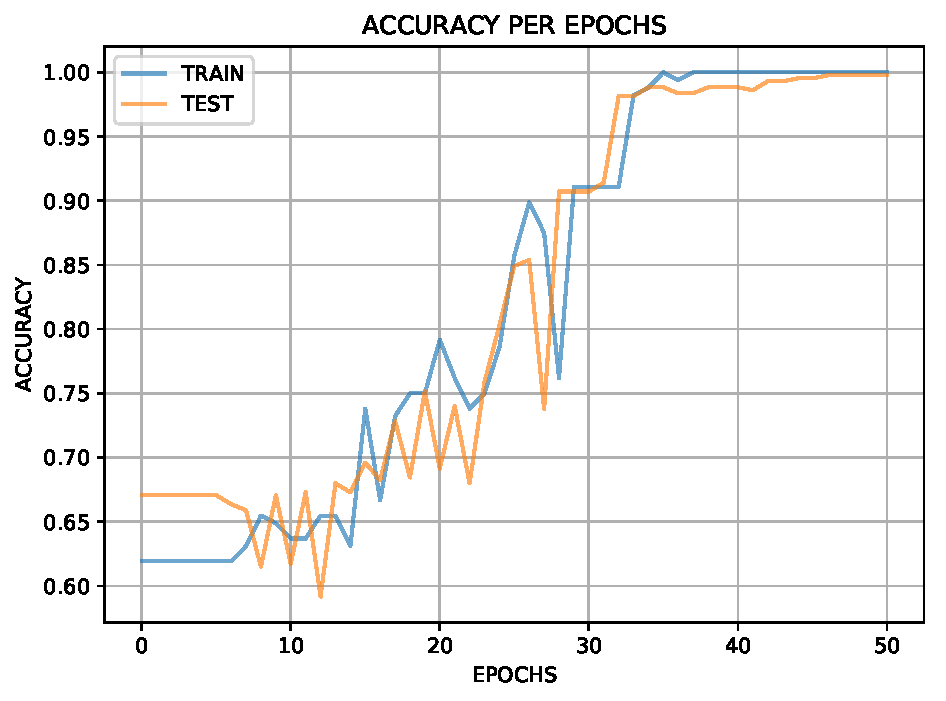
\includegraphics{img/CGD/MHS/cgd_accuracy_test_mhs_monks_2.pdf}
                    }
                    \caption{}
                    \label{fig:monks_2_ACC_CGD}
                \end{subfigure}
                \begin{subfigure}{0.40\textwidth}
                    \resizebox{\textwidth}{!}{
                        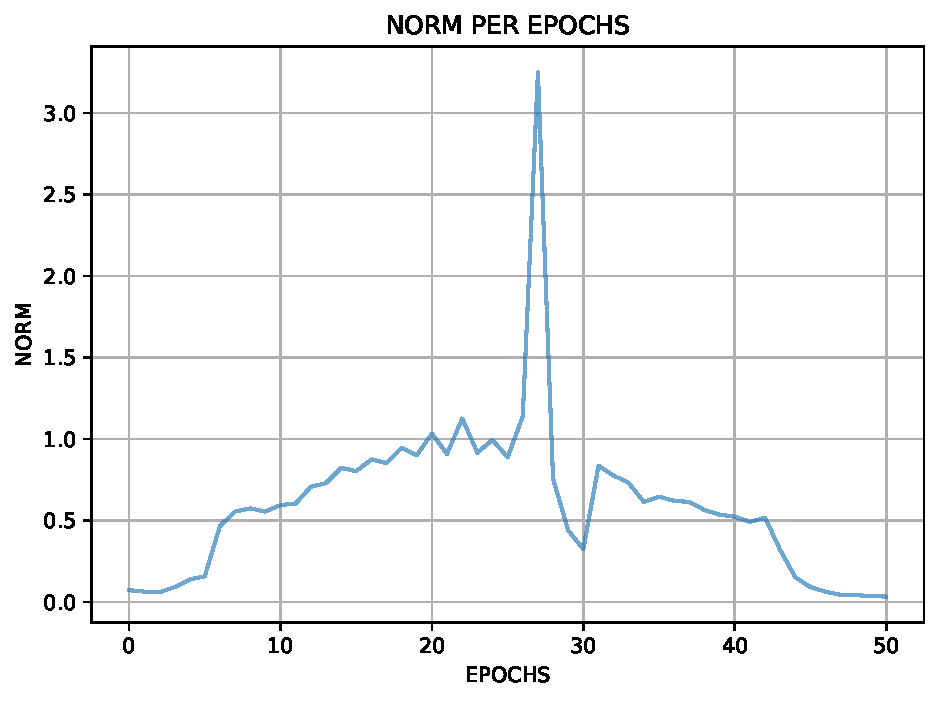
\includegraphics{img/CGD/MHS/cgd_norm_test_mhs_monks_2.pdf}
                    }
                    \caption{}
                    \label{fig:monks_2_NORM_CGD}
                \end{subfigure}
                \caption{Example of a final learning, accuracy score curve and
                convergence rate curve on MONKS 2  with $MHS^+$ method.}
                \label{fig:monks_2_CGD}
            \end{figure}

            \begin{figure}[H]
                \centering
                \begin{subfigure}{0.40\textwidth}
                    \resizebox{\textwidth}{!}{
                        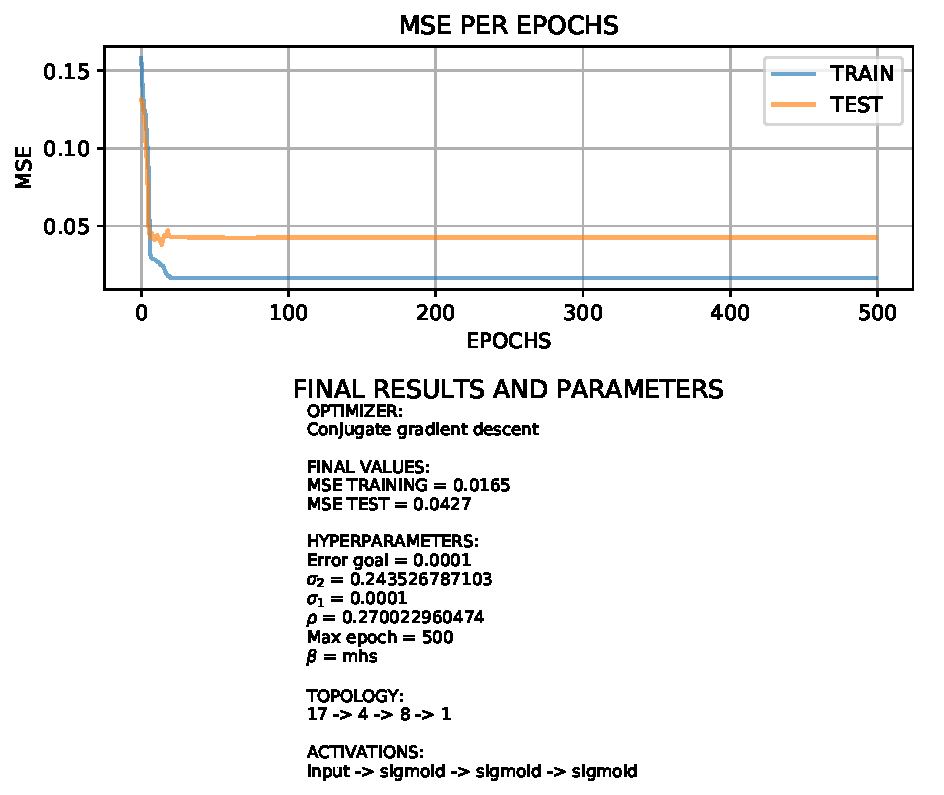
\includegraphics{img/CGD/MHS/cgd_mse_test_mhs_monks_3.pdf}
                    }
                    \caption{}
                    \label{fig:monks_3_MSE_CGD}
                \end{subfigure}
                \begin{subfigure}{0.40\textwidth}
                    \resizebox{\textwidth}{!}{
                        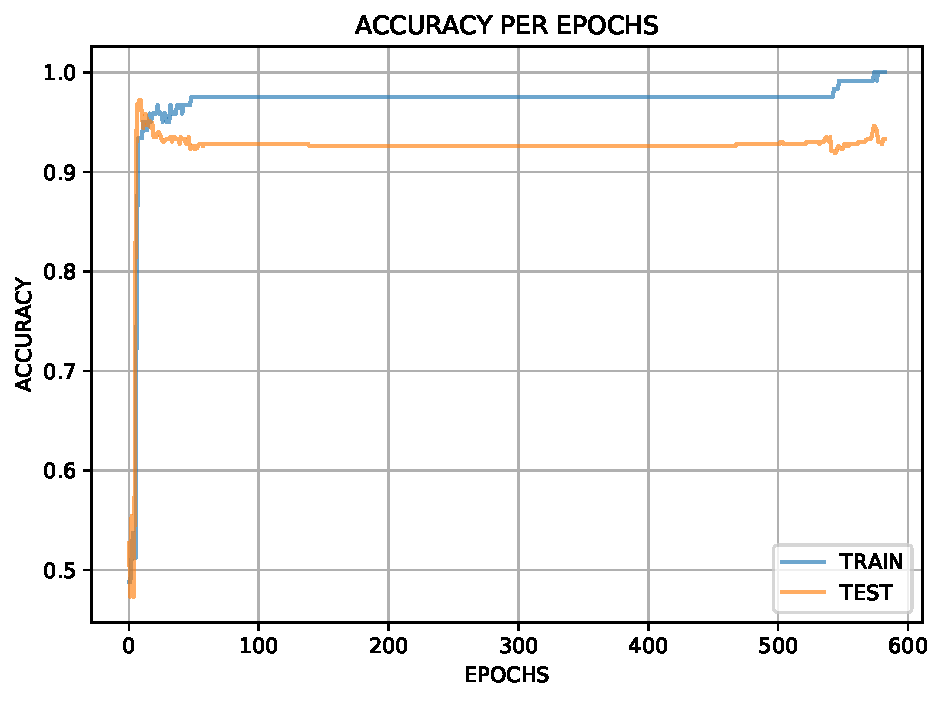
\includegraphics{img/CGD/MHS/cgd_accuracy_test_mhs_monks_3.pdf}
                    }
                    \caption{}
                    \label{fig:monks_3_ACC_CGD}
                \end{subfigure}
                \begin{subfigure}{0.40\textwidth}
                    \resizebox{\textwidth}{!}{
                        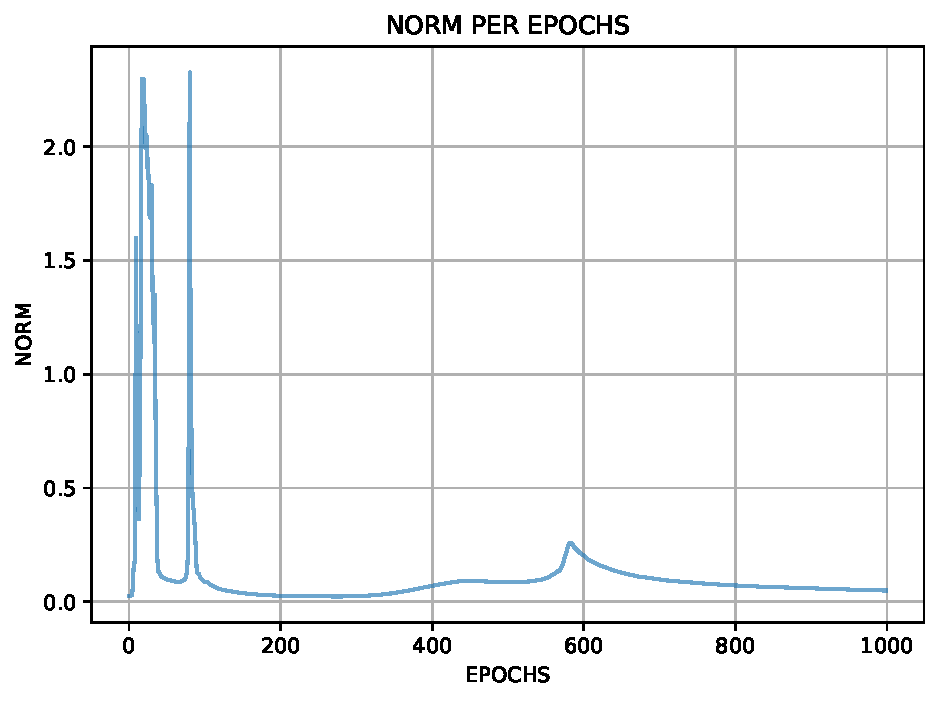
\includegraphics{img/CGD/MHS/cgd_norm_test_mhs_monks_3.pdf}
                    }
                    \caption{}
                    \label{fig:monks_3_NORM_CGD}
                \end{subfigure}
                \caption{Example of a final learning, accuracy score curve and
                convergence rate curve on MONKS 3 with $MHS^+$ method.}
                \label{fig:monks_3_CGD}
            \end{figure}



            % subsection mhs (end)

            \subsection{$HS^+$} % (fold)
            \label{sub:hs}

                \begin{figure}[H]
                \centering
                \begin{subfigure}{0.40\textwidth}
                    \resizebox{\textwidth}{!}{
                        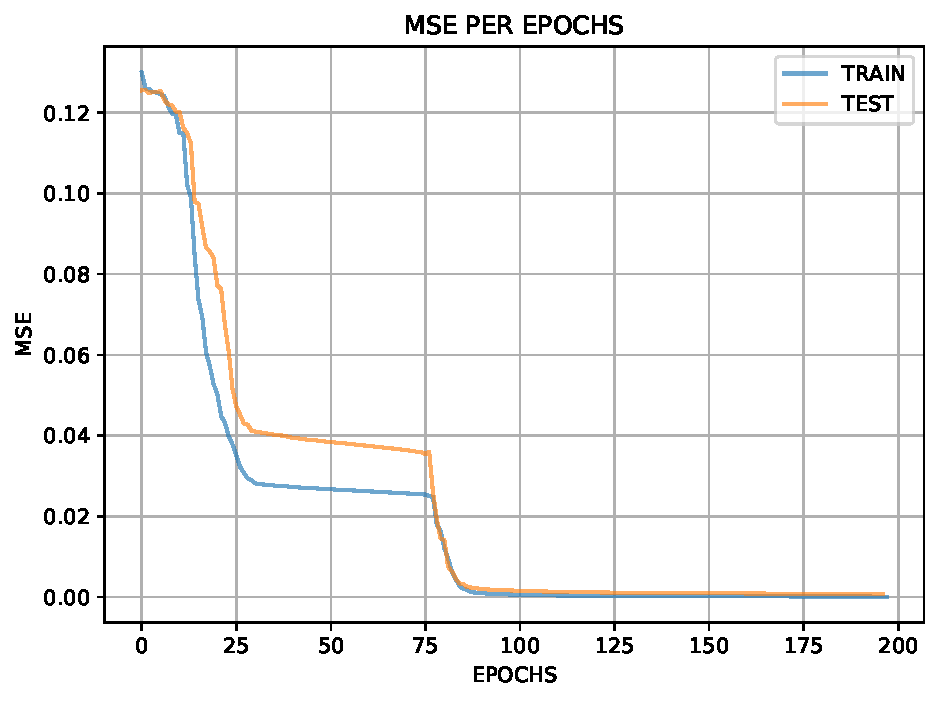
\includegraphics{img/CGD/HS/cgd_mse_test_hs_monks_1.pdf}
                    }
                    \caption{}
                    \label{fig:monks_1_MSE_CGD}
                \end{subfigure}
                \begin{subfigure}{0.40\textwidth}
                    \resizebox{\textwidth}{!}{
                        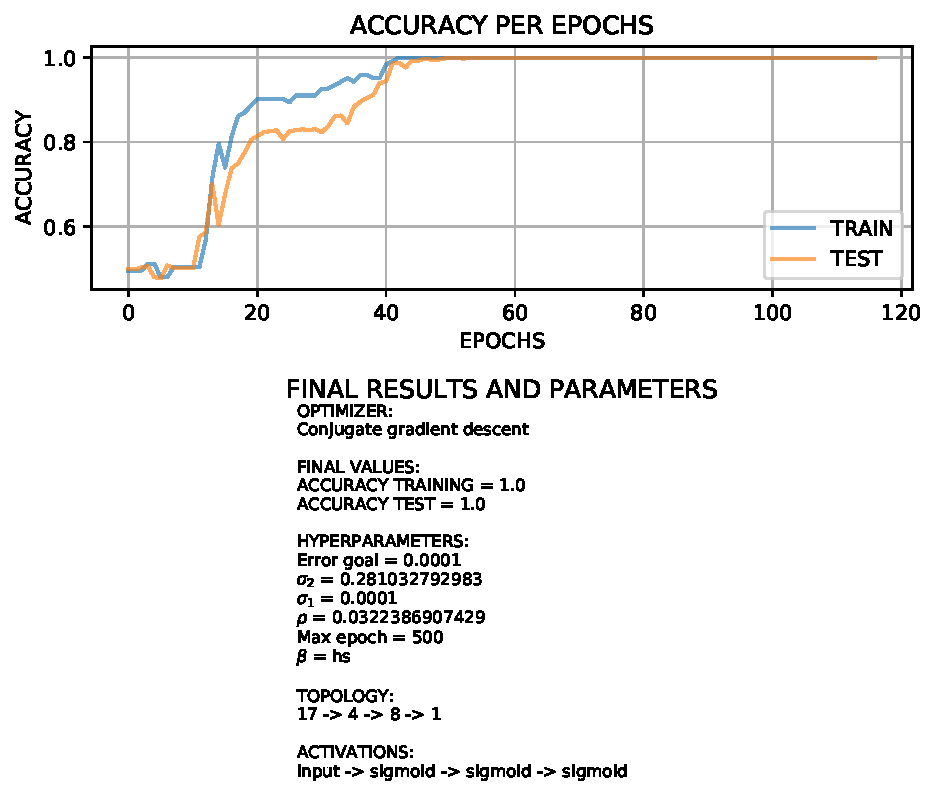
\includegraphics{img/CGD/HS/cgd_accuracy_test_hs_monks_1.pdf}
                    }
                    \caption{}
                    \label{fig:monks_1_ACC_CGD}
                \end{subfigure}
                \begin{subfigure}{0.40\textwidth}
                    \resizebox{\textwidth}{!}{
                        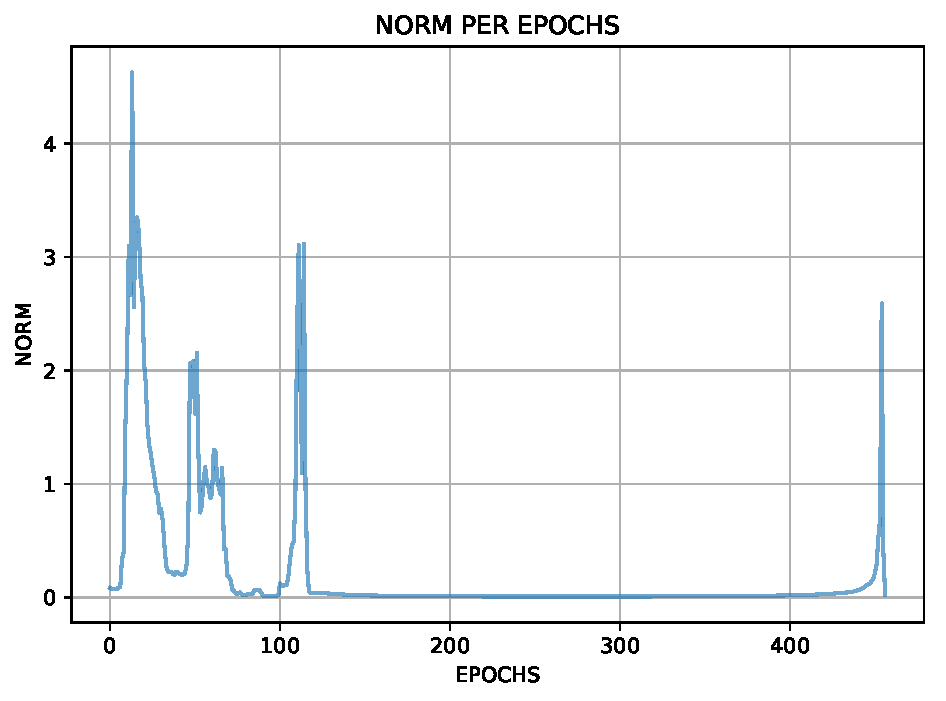
\includegraphics{img/CGD/HS/cgd_norm_test_hs_monks_1.pdf}
                    }
                    \caption{}
                    \label{fig:monks_1_NORM_CGD}
                \end{subfigure}
                \caption{Example of a final learning, accuracy score curve and
                convergence rate curve on MONKS 1 with $HS^+$ method.}
                \label{fig:monks_1_CGD}
            \end{figure}

            \begin{figure}[H]
                \centering
                \begin{subfigure}{0.40\textwidth}
                    \resizebox{\textwidth}{!}{
                        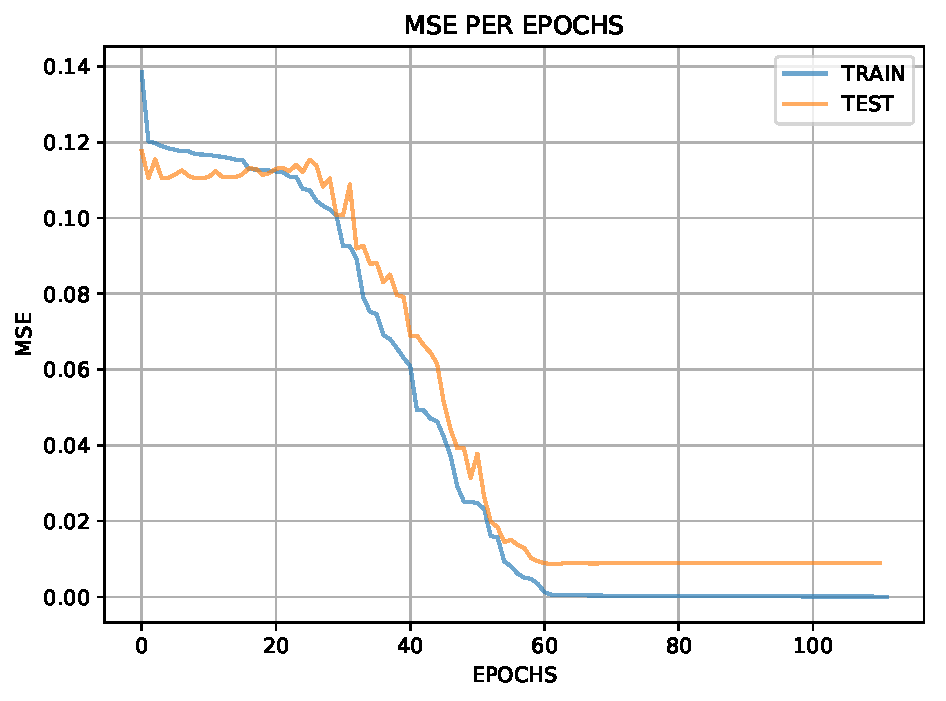
\includegraphics{img/CGD/HS/cgd_mse_test_hs_monks_2.pdf}
                    }
                    \caption{}
                    \label{fig:monks_2_MSE_CGD}
                \end{subfigure}
                \begin{subfigure}{0.40\textwidth}
                    \resizebox{\textwidth}{!}{
                        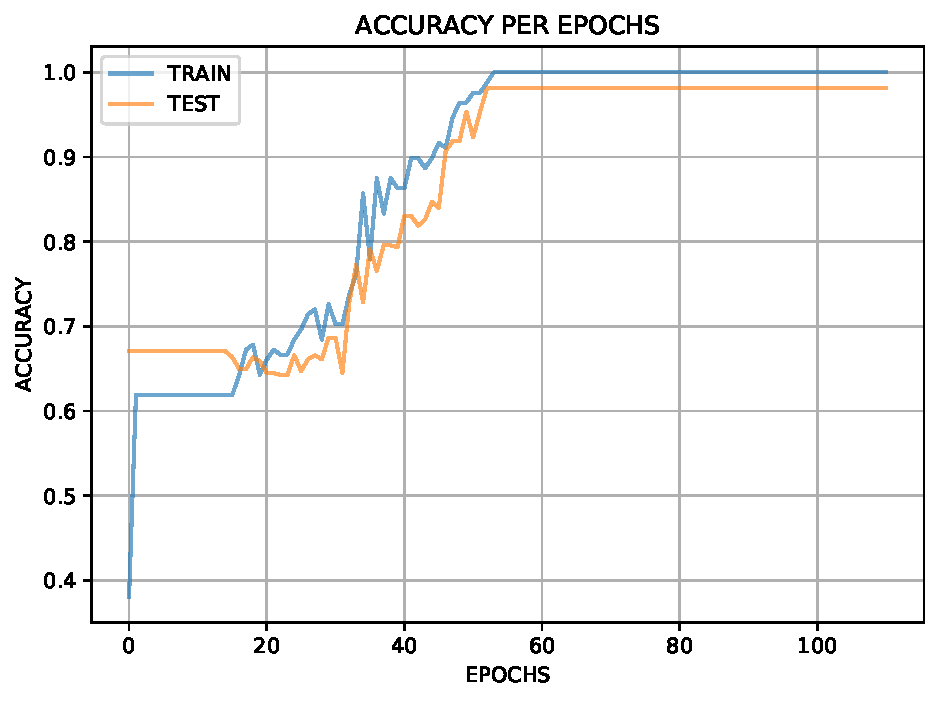
\includegraphics{img/CGD/HS/cgd_accuracy_test_hs_monks_2.pdf}
                    }
                    \caption{}
                    \label{fig:monks_2_ACC_CGD}
                \end{subfigure}
                \begin{subfigure}{0.40\textwidth}
                    \resizebox{\textwidth}{!}{
                        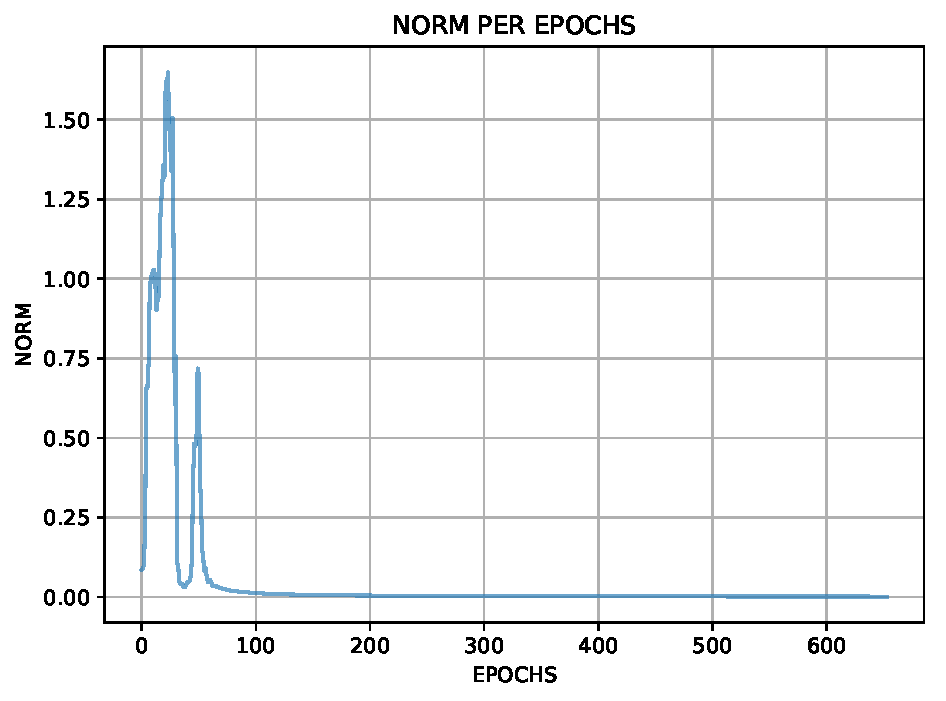
\includegraphics{img/CGD/HS/cgd_norm_test_hs_monks_2.pdf}
                    }
                    \caption{}
                    \label{fig:monks_2_NORM_CGD}
                \end{subfigure}
                \caption{Example of a final learning, accuracy score curve and
                convergence rate curve on MONKS 2  with $HS^+$ method.}
                \label{fig:monks_2_CGD}
            \end{figure}

            \begin{figure}[H]
                \centering
                \begin{subfigure}{0.40\textwidth}
                    \resizebox{\textwidth}{!}{
                        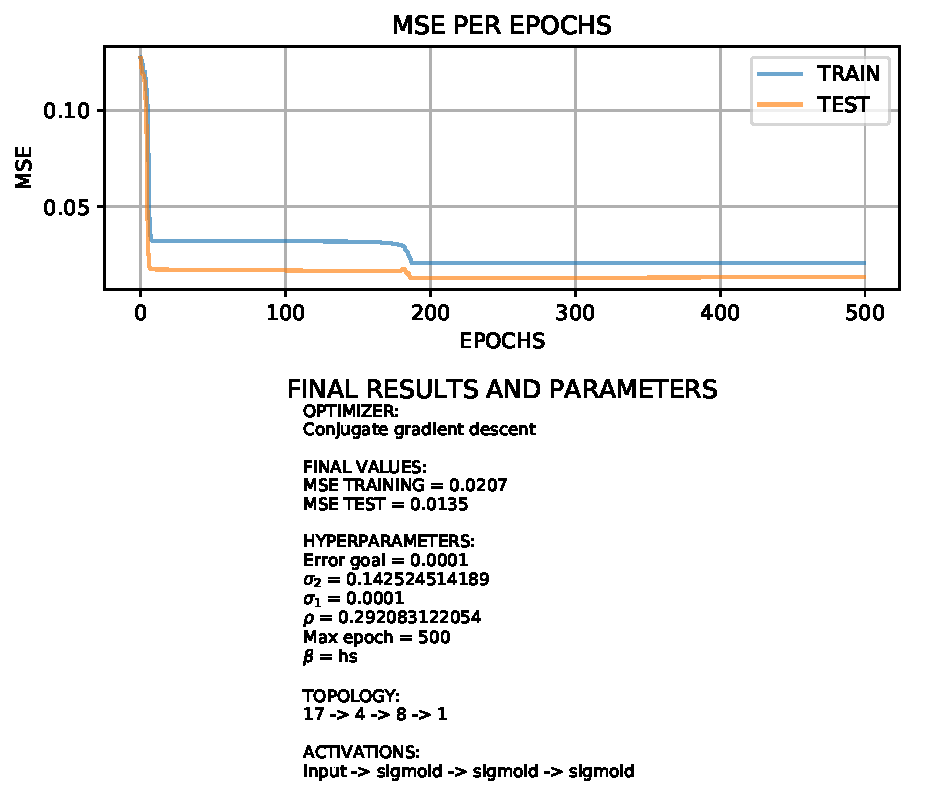
\includegraphics{img/CGD/HS/cgd_mse_test_hs_monks_3.pdf}
                    }
                    \caption{}
                    \label{fig:monks_3_MSE_CGD}
                \end{subfigure}
                \begin{subfigure}{0.40\textwidth}
                    \resizebox{\textwidth}{!}{
                        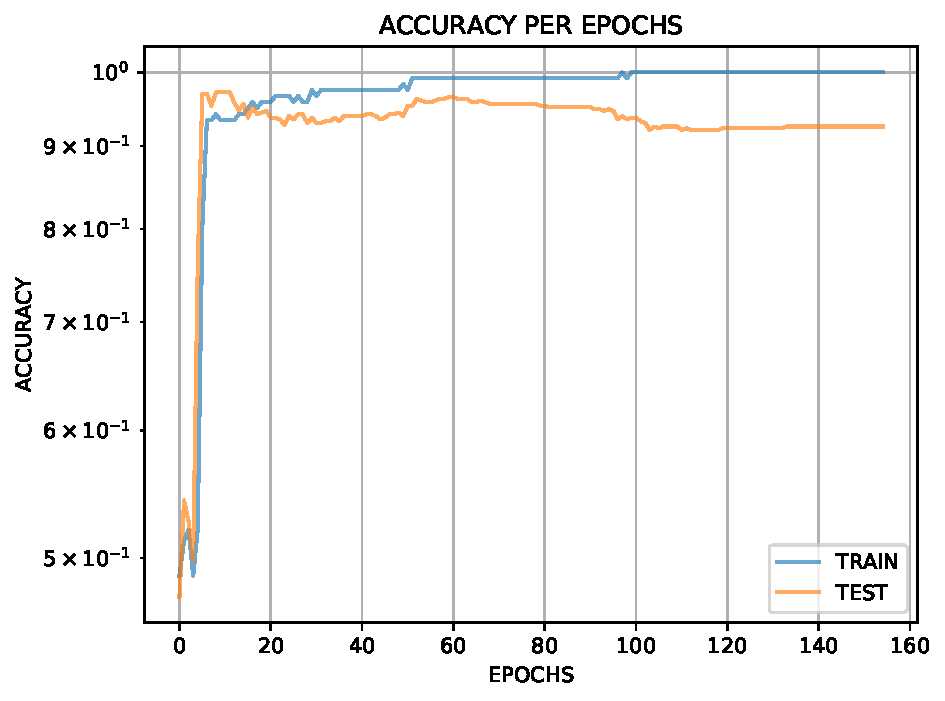
\includegraphics{img/CGD/HS/cgd_accuracy_test_hs_monks_3.pdf}
                    }
                    \caption{}
                    \label{fig:monks_3_ACC_CGD}
                \end{subfigure}
                \begin{subfigure}{0.40\textwidth}
                    \resizebox{\textwidth}{!}{
                        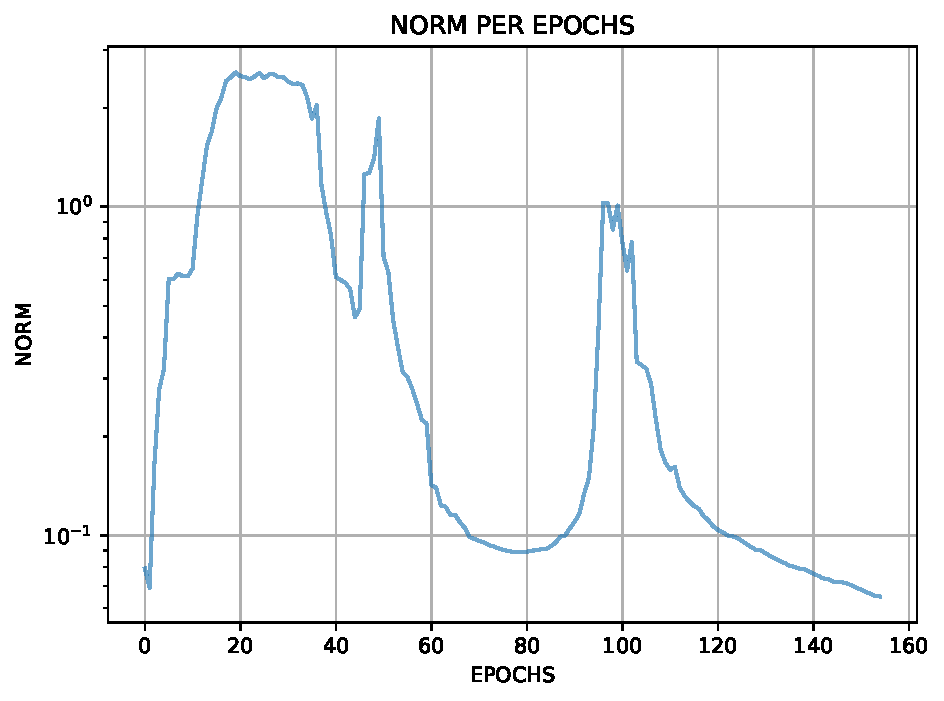
\includegraphics{img/CGD/HS/cgd_norm_test_hs_monks_3.pdf}
                    }
                    \caption{}
                    \label{fig:monks_3_NORM_CGD}
                \end{subfigure}
                \caption{Example of a final learning, accuracy score curve and
                convergence rate curve on MONKS 3 with $HS^+$ method.}
                \label{fig:monks_3_CGD}
            \end{figure}

            % subsection hs (end)

            \subsection{$PR^+$} % (fold)
            \label{sub:pr}

                \begin{figure}[H]
                \centering
                \begin{subfigure}{0.40\textwidth}
                    \resizebox{\textwidth}{!}{
                        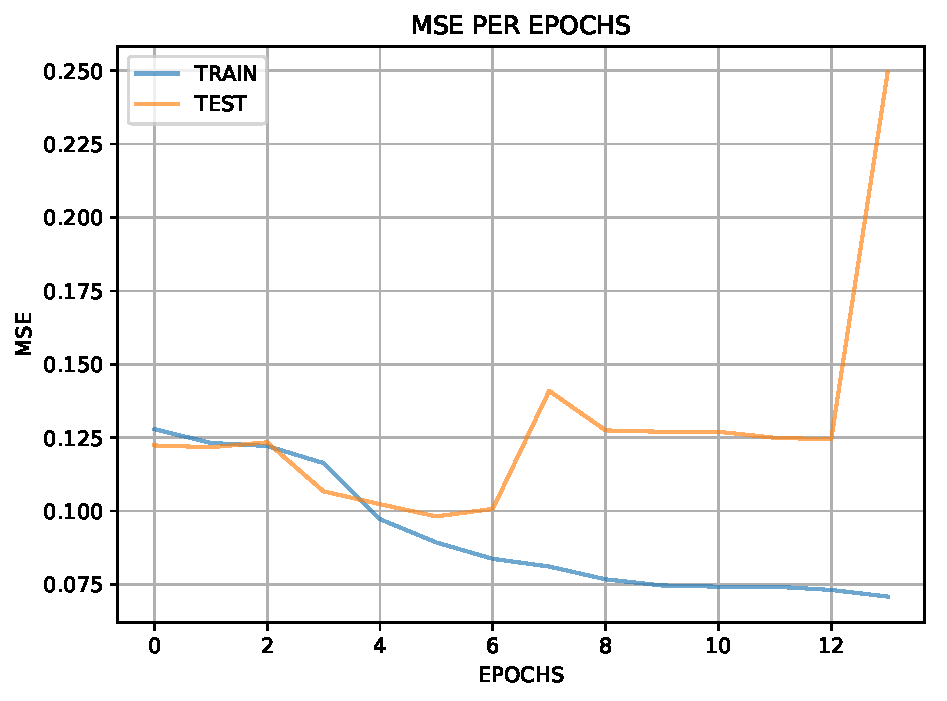
\includegraphics{img/CGD/PR/cgd_mse_test_pr_monks_1.pdf}
                    }
                    \caption{}
                    \label{fig:monks_1_MSE_CGD}
                \end{subfigure}
                \begin{subfigure}{0.40\textwidth}
                    \resizebox{\textwidth}{!}{
                        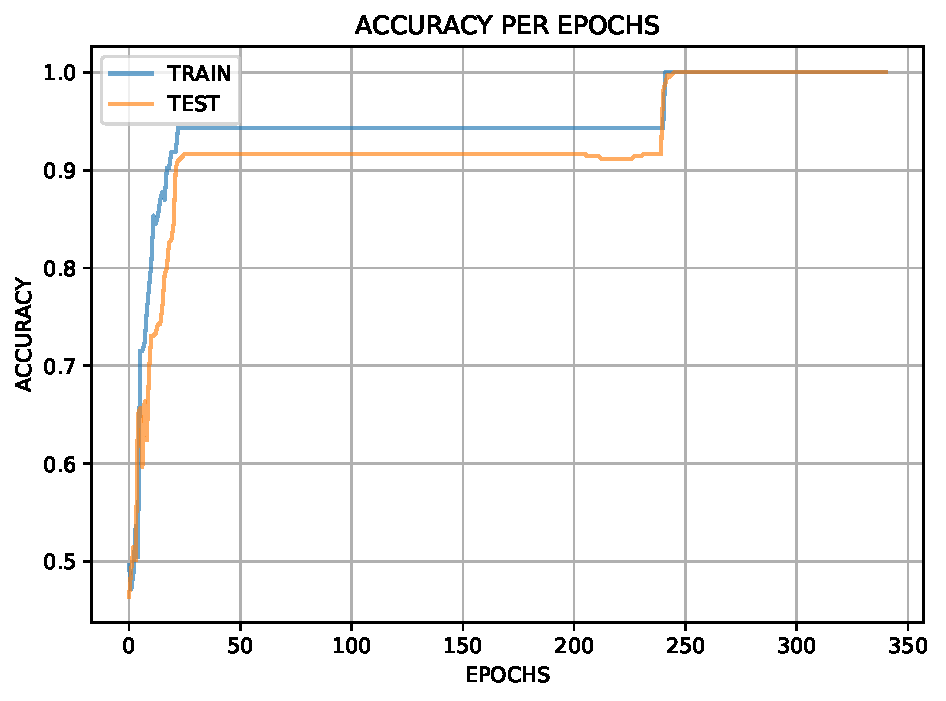
\includegraphics{img/CGD/PR/cgd_accuracy_test_pr_monks_1.pdf}
                    }
                    \caption{}
                    \label{fig:monks_1_ACC_CGD}
                \end{subfigure}
                \begin{subfigure}{0.40\textwidth}
                    \resizebox{\textwidth}{!}{
                        \includegraphics{img/CGD/PR/cgd_norm_test_pr_monks_1.pdf}
                    }
                    \caption{}
                    \label{fig:monks_1_NORM_CGD}
                \end{subfigure}
                \caption{Example of a final learning, accuracy score curve and
                convergence rate curve on MONKS 1 with $PR^+$ method.}
                \label{fig:monks_1_CGD}
            \end{figure}

            \begin{figure}[H]
                \centering
                \begin{subfigure}{0.40\textwidth}
                    \resizebox{\textwidth}{!}{
                        \includegraphics{img/CGD/PR/cgd_mse_test_pr_monks_2.pdf}
                    }
                    \caption{}
                    \label{fig:monks_2_MSE_CGD}
                \end{subfigure}
                \begin{subfigure}{0.40\textwidth}
                    \resizebox{\textwidth}{!}{
                        \includegraphics{img/CGD/PR/cgd_accuracy_test_pr_monks_2.pdf}
                    }
                    \caption{}
                    \label{fig:monks_2_ACC_CGD}
                \end{subfigure}
                \begin{subfigure}{0.40\textwidth}
                    \resizebox{\textwidth}{!}{
                        \includegraphics{img/CGD/PR/cgd_norm_test_pr_monks_2.pdf}
                    }
                    \caption{}
                    \label{fig:monks_2_NORM_CGD}
                \end{subfigure}
                \caption{Example of a final learning, accuracy score curve and
                convergence rate curve on MONKS 2  with $PR^+$ method.}
                \label{fig:monks_2_CGD}
            \end{figure}

            \begin{figure}[H]
                \centering
                \begin{subfigure}{0.40\textwidth}
                    \resizebox{\textwidth}{!}{
                        \includegraphics{img/CGD/PR/cgd_mse_test_pr_monks_3.pdf}
                    }
                    \caption{}
                    \label{fig:monks_3_MSE_CGD}
                \end{subfigure}
                \begin{subfigure}{0.40\textwidth}
                    \resizebox{\textwidth}{!}{
                        \includegraphics{img/CGD/PR/cgd_accuracy_test_pr_monks_3.pdf}
                    }
                    \caption{}
                    \label{fig:monks_3_ACC_CGD}
                \end{subfigure}
                \begin{subfigure}{0.40\textwidth}
                    \resizebox{\textwidth}{!}{
                        \includegraphics{img/CGD/PR/cgd_norm_test_pr_monks_3.pdf}
                    }
                    \caption{}
                    \label{fig:monks_3_NORM_CGD}
                \end{subfigure}
                \caption{Example of a final learning, accuracy score curve and
                convergence rate curve on MONKS 3 with $PR^+$ method.}
                \label{fig:monks_3_CGD}
            \end{figure}

            % subsection pr (end)

        % section conjugate_gradient_methods (end)

    % chapter monks_learning_curves (end)

    \chapter{CUP's learning curves} % (fold)
    \label{cha:cup_learning_curves}
        As in the previous section, the following curves are the result of the final tests on the test dataset. It has been plotted one of the 10 trails we used for building the statistics we presented in Section \ref{sec:cup}, hence each plot presents a possible learning curve for the best hyperparameters’ selection for each dataset.
        \section{Stochastic Gradient Descent} % (fold)
        \label{sec:cup_sgd}

        %     \begin{figure}[H]
        %         \centering
        %             \resizebox{\textwidth}{!}{
        %                 \includegraphics{img/SGD/sgd_mse_test_cup.pdf}
        %             }
        %             \label{fig:cup_MSE_SGD}
        %         \caption{Example of a final learning curve on CUP.}
        %         \label{fig:cup_SGD}
        %     \end{figure}

        % \section{Conjugate Gradient Methods}
        % \label{sec:cgd}
        %     \subsection{$MHS^+$}
        %     \label{sec:cup_msh}

        %         \begin{figure}[H]
        %             \centering
        %                 \resizebox{\textwidth}{!}{
        %                     \includegraphics{img/CGD/MHS/cgd_mse_test_mhs_cup.pdf}
        %                 }
        %                 \label{fig:cup_mhs}
        %             \caption{Example of a final learning curve on CUP.}
        %         \end{figure}

        %     \subsection{$HS^+$}
        %     \label{sec:cup_hs}

        %         \begin{figure}[H]
        %             \centering
        %                 \resizebox{\textwidth}{!}{
        %                     \includegraphics{img/CGD/MHS/cgd_mse_test_hs_cup.pdf}
        %                 }
        %                 \label{fig:cup_hs}
        %             \caption{Example of a final learning curve on CUP.}
        %         \end{figure}

        %     \subsection{$PR^+$}
        %     \label{sec:cup_pr}

        %         \begin{figure}[H]
        %             \centering
        %                 \resizebox{\textwidth}{!}{
        %                     \includegraphics{img/CGD/MHS/cgd_mse_test_pr_cup.pdf}
        %                 }
        %                 \label{fig:cup_pr}
        %             \caption{Example of a final learning curve on CUP.}
        %         \end{figure}
        % % section sgd (end)

\end{appendices}
